\ifdefined\ishandout
\documentclass[handout]{beamer}
\else
\documentclass{beamer}
\fi

%\usepackage[frenchb]{babel}
\usepackage[T1]{fontenc}
%\usepackage[utf8]{inputenc}
\usepackage{hyperref}
\usepackage{multirow}
\usepackage{listings}
\usepackage{fancyvrb}
\usepackage{tikz}
\usepackage{framed}
\usepackage{xmpmulti}

\usepackage{algorithm}
\usepackage{algorithmicx}
\usepackage{algpseudocode}
\usepackage{xcolor}
\usepackage{booktabs}
\usepackage{color, colortbl}
\ifdefined\ishandout
\usepackage{handoutWithNotes}
\fi
\usepackage{slashbox}
\usepackage{amsmath}
\usepackage{bm}
\usepackage{hhline}
\usepackage{pgfplots}
\usepackage{caption}

\def\UrlBreaks{\do\/\do-}

\usetikzlibrary{shapes.geometric}
\usetikzlibrary{positioning}
\usetikzlibrary{shapes.arrows, chains}
\usetikzlibrary{arrows,calc}
\usetikzlibrary{shapes.multipart}
\usetikzlibrary{matrix}

\usepackage{array}
%\usetheme{Boadilla}
\usetheme[progressbar=frametitle]{metropolis}

\usefonttheme[onlymath]{serif}

\newcommand{\R}{\mathbb{R}}
%\newcommand{\C}{\mathbb{C}}
\newcommand{\N}{\mathbb{N}}
\newcommand{\Z}{\mathbb{Z}}
\newcommand{\E}{\mathbb{E}}
\newcommand{\Var}{\text{Var}}
\newcommand{\Cov}{\text{Cov}}
\ifdefined\ishandout
\pgfpagesuselayout{3 on 1 with notes}[a4paper,border shrink=5mm]
\usecolortheme{dove}
\else
%\usecolortheme{dolphin}
%\usecolortheme{crane}
\fi

\metroset{block=fill}

\lstnewenvironment{codeC}
{ \lstset{language=C,
    otherkeywords={printf,scanf}}
}
{}

\ifdefined\ishandout
\definecolor{mygreen}{rgb}{0,0,0}
\definecolor{mymauve}{rgb}{0,0,0}
\definecolor{myblue}{rgb}{0,0,0}
\else
\definecolor{mygreen}{rgb}{0,0.6,0}
\definecolor{mymauve}{rgb}{0.58,0,0.82}
\definecolor{myblue}{rgb}{0,0,1}

\fi

%% Notes
%\setbeameroption{show only notes}


\definecolor{mygray}{rgb}{0.5,0.5,0.5}

\lstset{ language=Python,%
  backgroundcolor=\color{white},   % choose the background color; you must add \usepackage{color} or \usepackage{xcolor}
  basicstyle=\footnotesize,        % the size of the fonts that are used for the code
  breakatwhitespace=false,         % sets if automatic breaks should only happen at whitespace
  breaklines=true,                 % sets automatic line breaking
  captionpos=b,                    % sets the caption-position to bottom
  commentstyle=\color{mygreen},    % comment style
  deletekeywords={...},            % if you want to delete keywords from the given language
  escapeinside={\%*}{*)},          % if you want to add LaTeX within your code
  extendedchars=true,              % lets you use non-ASCII characters; for 8-bits encodings only, does not work with UTF-8
  frame=tb,	                   % adds a frame around the code
  keepspaces=true,                 % keeps spaces in text, useful for keeping indentation of code (possibly needs columns=flexible)
  keywordstyle=\color{blue},       % keyword style
  otherkeywords={*,...},           % if you want to add more keywords to the set
  numbers=none,                    % where to put the line-numbers; possible values are (none, left, right)
  numbersep=5pt,                   % how far the line-numbers are from the code
  numberstyle=\tiny\color{mygray}, % the style that is used for the line-numbers
  rulecolor=\color{black},         % if not set, the frame-color may be changed on line-breaks within not-black text (e.g. comments (green here))
  showspaces=false,                % show spaces everywhere adding particular underscores; it overrides 'showstringspaces'
  showstringspaces=false,          % underline spaces within strings only
  showtabs=false,                  % show tabs within strings adding particular underscores
  stepnumber=2,                    % the step between two line-numbers. If it's 1, each line will be numbered
  stringstyle=\color{mymauve},     % string literal style
  tabsize=3,	                   % sets default tabsize to 2 spaces
  title=\lstname                   % show the filename of files included with \lstinputlisting; also try caption instead of title
}
%\lstset{language=Python,
% breakatwhitespace=false,         % sets if automatic breaks should only happen at whitespace
%  breaklines=true,                 % sets automatic line breaking
%  captionpos=b,                
%%commentstyle=\itshape\color{mymauve},
%%keywordstyle=\bfseries\color{myblue},
%numbers=left,                    % where to put the line-numbers; possible values are (none, left, right)
%  numbersep=8pt,                   % how far the line-numbers are from the code
%  numberstyle=\tiny\color{mygray}, % the style that is used for the line-numbers
%%  rulecolor=\color{black},         % if not set, the frame-color may be changed on line-breaks within not-black text (e.g. comments (green here))
%  showspaces=false,                % show spaces everywhere adding particular underscores; it overrides 'showstringspaces'
%%  showstringspaces=false,          % underline spaces within strings only
%  showtabs=false,                  % show tabs within strings adding particular underscores
%  stepnumber=2,                    % the step between two line-numbers. If it's 1, each line will be numbered
%%  stringstyle=\color{mygreen},     % string literal style
%  tabsize=2 
%}
\ifdefined\ishandout
\newcommand{\red}{\textbf}
\else
\newcommand{\red}{\textcolor{red}}
\fi
%\newcommand \emph
%Default size : 12.8 cm * 9.6 cm

\newcommand{\tmark}[1]{\tikz[remember picture, baseline=-.5ex]{\coordinate(#1);}}

\definecolor{bluegreen}{RGB}{0,149,182}


%\newcommand{\output}[1]{
\setbeamertemplate{navigation symbols}{}
\newcommand{\bvrb}{\Verb[commandchars=£µ§,formatcom=\color{bluegreen}]}
\newcommand{\footvrb}{\footnotesize\Verb}
\newcommand{\vrbalert}[2][]{\visible<#1>{#2}}
%%% Commande pour les listes/arbres
\newcommand{\mvide}{\nodepart{one} \nodepart{two}}
\newcommand{\tvide}{\nodepart{one} \nodepart{two} \nodepart{three}}
\newcommand{\rref}[1][]{\hfill{\scriptsize\textit{#1}}}

%%Fin des commandes pour les listes/arbres.



%%% Paramètres du cours (à régler)
%Numéro du cours
\newcommand{\nb}{1}

\title[Machine Learning]{Machine learning and physical modelling-2}
\author[J. Brajard]{julien.brajard@nersc.no}
\institute[NERSC]{NERSC\\
\url{https://github.com/brajard/MAT330}}
\date{October 2022}

\begin{document}
%%%%%%%%%%%%%%%%%%%%% SLIDES DE TITRE
\begin{frame}
\titlepage
%\centering{
%\url{http://australe.upmc.fr} (onglet EPU-C5-IGE Info Gen)}
\end{frame}

\begin{frame}{Table of contents}
  \setbeamertemplate{section in toc}[sections numbered]
  \tableofcontents[hideallsubsections]
\end{frame}

\section{A standard Machine learning model: Random Forests}


%%%%%%%%%%%%%%%%%%%%%%%%%%%%%%%%%%%%%%%%%%
\begin{frame}{A decision tree}
    Predict house price (in \$100,000) from 8 features:
    \begin{figure}
        \centering
        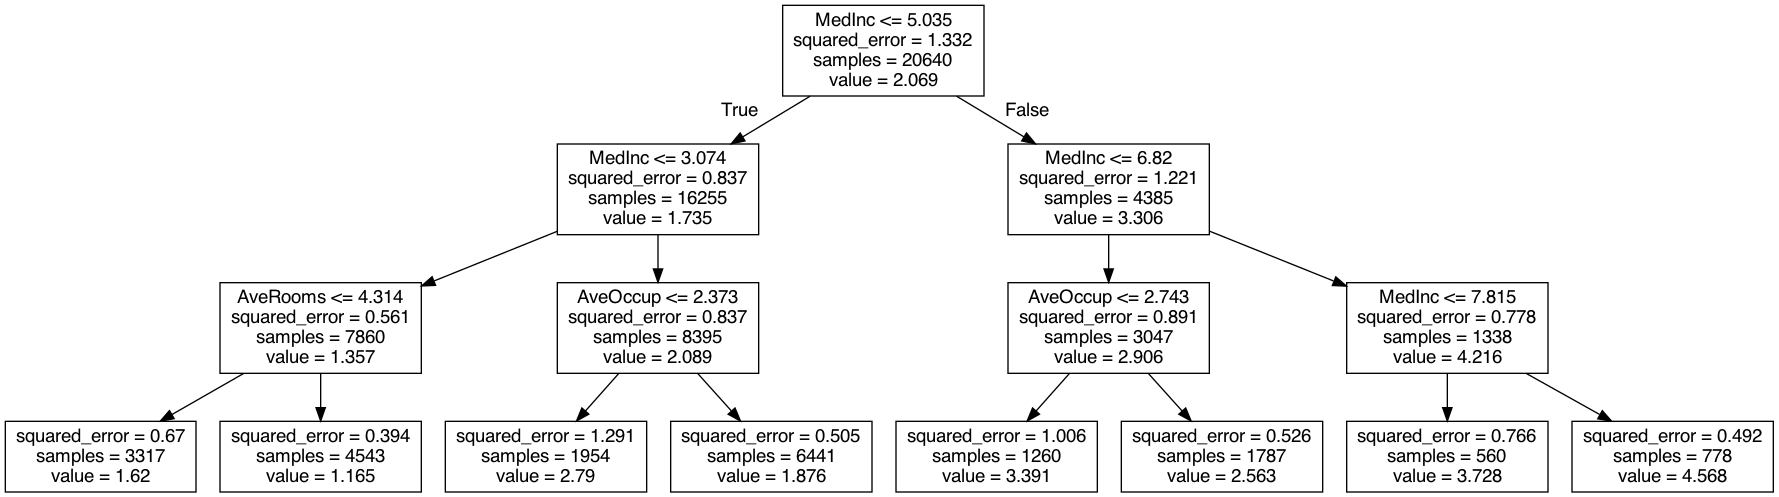
\includegraphics[width=\textwidth]{fig/L2/tree.png}
    \end{figure}
        
    \begin{table}
    \centering
    \begin{tabular}{c|l}
    MedInc & median income in block group \\
    AveRooms & average number of rooms per household \\
    AveOccup   &   average number of household members \\
    ... & ...\\
        \end{tabular}
        \end{table}

\end{frame}

%%%%%%%%%%%%%%%%%%%%%%%%%%%%%%%%%%%%%%%%%%
\begin{frame}{Uni-variate example}
\begin{columns}
\column{.5\textwidth}
\begin{figure}
    \centering
    \includegraphics<1>[width=\textwidth]{fig/L2/tree-data.png}
    \includegraphics<2>[width=\textwidth]{fig/L2/tree-2.png}
    \includegraphics<3>[width=\textwidth]{fig/L2/tree-5.png}
\end{figure}
    \column{.5\textwidth}
\begin{figure}
    \centering
    \includegraphics<2>[width=\textwidth]{fig/L2/tree_uni_2.png}
    \includegraphics<3>[width=\textwidth]{fig/L2/tree_uni_5.png}
\end{figure}
\end{columns}

\end{frame}

%%%%%%%%%%%%%%%%%%%%%%%%%%%%%%%%%%%%%%%%%%
\begin{frame}{From tree to forest}
Disadvantages of regression tree:
\begin{itemize}
    \item Can overfit the data
\end{itemize}
\visible<2->{
One extension of Regression Tree:
\alert{Random Forest}}
\begin{figure}
    \centering
    \includegraphics<1>[width=.7\textwidth]{fig/L2/tree.jpg}
    \includegraphics<2>[width=.7\textwidth]{fig/L2/forest.jpeg}
\end{figure}
\end{frame}

%%%%%%%%%%%%%%%%%%%%%%%%%%%%%%%%%%%%%%%%%%
\begin{frame}{The (over simplified) principle of Random Forest}
\begin{tikzpicture}[node distance = 0.5 cm]
\draw [very thick, fill=gray] (0,0) rectangle (3,6);
\node (data) at (1.5,6.2) {Data};
\pause
%TREE 1
\def\xx{4}
\def\yy{4.5}
\foreach \y in {0.5,2,3,3.5,4.5}
{
\draw[orange,fill=orange] (0,\y) rectangle +(3,.5);
}
\draw [very thick] (0,0) rectangle (3,6);

\draw [black,fill=orange] (\xx,\yy) rectangle +(1,1.5);
\path [->,draw] (3,3) -- (\xx,{\yy + 0.75});
\pause
\node [anchor=west] (t1) at ({\xx+2},{\yy + 0.75}) {Tree 1};
\path [->,draw] ({\xx+1},{\yy + 0.75}) -- node [above] {fit} ({\xx+2},{\yy + 0.75}) ;

\pause
%TREE 2
\def\xx{4}
\def\yy{2.5}

\draw [very thick, fill=gray] (0,0) rectangle (3,6);

\foreach \y in {0.,1,2,2.5,3.5,4.5}
{
\draw[blue,fill=blue] (0,\y) rectangle +(3,.5);
}
\draw [very thick] (0,0) rectangle (3,6);

\draw [black,fill=blue] (\xx,\yy) rectangle +(1,1.5);
\path [->,draw] (3,3) -- (\xx,{\yy + 0.75});
\node [anchor=west] (t2) at ({\xx+2},{\yy + 0.75}) {Tree 2};
\path [->,draw] ({\xx+1},{\yy + 0.75}) -- node [above] {fit} ({\xx+2},{\yy + 0.75}) ;

\pause
%TREE 3
\def\xx{4}
\def\yy{0.5}

\draw [very thick, fill=gray] (0,0) rectangle (3,6);

\foreach \y in {0.5,1.5,2,3.5,5.5}
{
\draw[red,fill=red] (0,\y) rectangle +(3,.5);
}
\draw [very thick] (0,0) rectangle (3,6);

\draw [black,fill=red] (\xx,\yy) rectangle +(1,1.5);
\path [->,draw] (3,3) -- (\xx,{\yy + 0.75});
\node [anchor=west] (t3)  at ({\xx+2},{\yy + 0.75}) {Tree 3};
\path [->,draw] ({\xx+1},{\yy + 0.75}) -- node [above] {fit} ({\xx+2},{\yy + 0.75}) ;

\pause
\node [right = of t2](average) {\textbf{Average}};
\node [right = of average] (out) {};
\path[->,draw] (t1) -- (average) ;
\path[->,draw] (t2) -- (average) ;
\path[->,draw] (t3) -- (average) ;
\path[->,draw] (average) -- (out) ;

\end{tikzpicture}
\end{frame}
%%%%%%%%%%%%%%%%%%%%%%%%%%%%%%%%%%%%%%%%%%
\begin{frame}{Results on the univariate experiment}

\begin{figure}
    \centering
\caption*{
\alt<1>{Prediction of Randoms trees}{Prediction of a Random Forest}}
    \includegraphics<1>[width=.9\textwidth]{fig/L2/tree-5.png}
    \includegraphics<2>[width=.9\textwidth]{fig/L2/RF.png}

\end{figure}


\end{frame}

%%%%%%%%%%%%%%%%%%%%%%%%%%%%%%%%%%%%%%%%%%
\begin{frame}[fragile]{Feature importance}
\begin{lstlisting}[language=Python]
rf = RandomForestRegressor(n_estimators=1000,max_features=10,random_state=10)
rf.fit(X,y)
importances = rf.feature_importances_
\end{lstlisting}
\vspace{-1.5em}
Indicates the impact of a feature in predicting the target.
\begin{columns}
\column{.5\textwidth}
    \begin{figure}
        \centering
        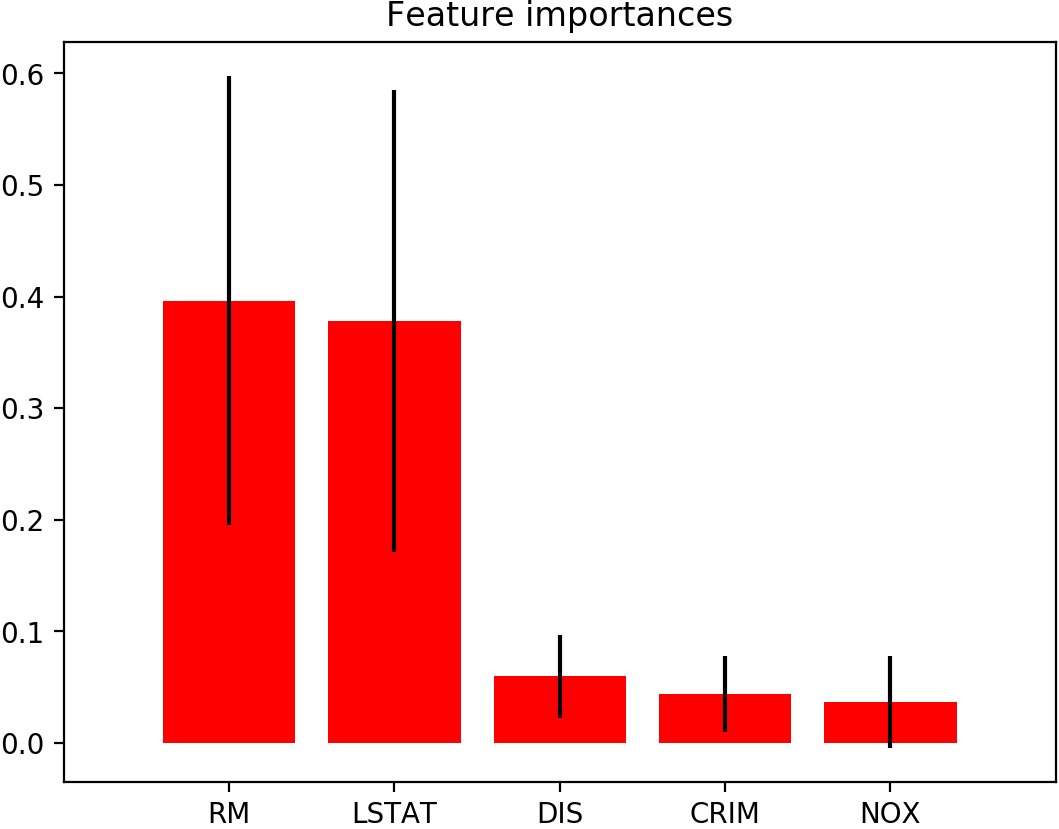
\includegraphics[width=.9\textwidth]{fig/L2/importance_RF.png}
    \end{figure}
\column{.5\textwidth}
    \begin{table}
    \centering
    \footnotesize
    \begin{tabular}{c|p{4.5cm}}
    MedInc & median income in block group \\
    AveRooms & average number of rooms per household \\
    AveOccup   &   average number of household members \\
    ... & ...\\
        \end{tabular}
        \end{table}

\end{columns}
\end{frame}

%%%%%%%%%%%%%%%%%%%%%%%%%%%%%%%%%%%%%%%%%%
\begin{frame}[fragile]{Some key parameters}
\begin{lstlisting}[language=Python]
from sklearn.ensemble import RandomForestClassifier

rf = RandomForestRegressor(n_estimators=n, max_features=maxf, min_samples_split=min_split,...)
\end{lstlisting}
\vspace{-1.5em}
\begin{itemize}[<+->]
    \item \verb|n_estimators|: number of trees (generally the larger is the better)
    \item   \verb|max_features|: number of features to consider at each split. The default number is the total number of features. A larger value makes provides a smaller bias (accuracy) but a bigger variance (risk of overfitting)
      \item \verb|min_samples_fit|: minimum number of features to consider at each split. The minimum value of 2 means that the tree is fully developed (small bias but great variance).
\end{itemize}

\end{frame}




%%%%%%%%%%%%%%%%%%%%%%%%%%%%%%%%%%%%%%%%%%
\begin{frame}{Determination of the hyperparameters}
    \begin{itemize}[<+->]
        \item Parameters that are not optimized during the training are called \alert{hyperparameters}.
        \item They can be determined using a score on the \alert{validation dataset} or using a \alert{cross-validation} procedure.
    \end{itemize}
    \pause
    \begin{columns}[b]
    \column{.42\textwidth}
      \begin{figure}
       \centering
       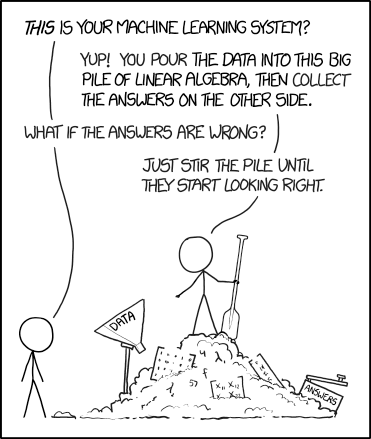
\includegraphics[width=\textwidth]{fig/L2/machine_learning.png}
   \end{figure}
   \column{.58\textwidth}
   \vfill
   {\footnotesize
   \url{https://xkcd.com/1838/}}
    \end{columns}

\end{frame}

%%%%%%%%%%%%%%%%%%%%%%%%%%%%%%%%%%%%%%%%%%
\begin{frame}{Stir the pile: The gridsearch}
\begin{enumerate}
    \item Specify a list of hyperparameters to be tested.
    \item For each of the parameters, specify a set of values to test
    \item Train a model for each of the possible combinations of hyperparameters
    \item Retain the best model (using, e.g., cross-validation)
\end{enumerate}

\begin{columns}[b]
\column{.5\textwidth}
\begin{figure}
    \centering
    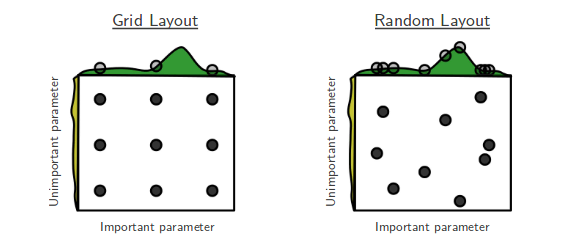
\includegraphics[trim={0 0 10cm 0},clip,width=\textwidth]{fig/L2/cIDuR.png}
\end{figure}
\column{.5\textwidth}

\vfill
{\footnotesize \url{https://medium.com/@senapati.dipak97/grid-search-vs-random-search-d34c92946318}
}
\end{columns}



\end{frame}

%%%%%%%%%%%%%%%%%%%%%%%%%%%%%%%%%%%%%%%%%%
\begin{frame}{Remarks on the gridsearch procedure}

\begin{itemize}[<+->]
    \item It make an \alert{exhaustive} search of the hyperparameters
    \item The procedure is easy to \alert{parallelized}.
    \item it is not naturally adapted for quantitative hyperparameters.
    \item it can become \alert{very costly}. (e.g. 8 hyperparameters with 8 values each to test = $8^8=16,777,216$ trainings.
\end{itemize}

\end{frame}


%%%%%%%%%%%%%%%%%%%%%%%%%%%%%%%%%%%%%%%%%%
\begin{frame}{Random search}
    \begin{enumerate}
    \item Specify a list of hyperparameters to be tested.
    \item For each of the parameters, specify a set of values to test or a law to draw a random value.
    \item Draw $n$ combinations of the hyperparameters.
    \item Train a model for each of the combinations.
    \item Retain the best model (using, e.g., cross-validation)
\end{enumerate}
\begin{figure}
    \centering
    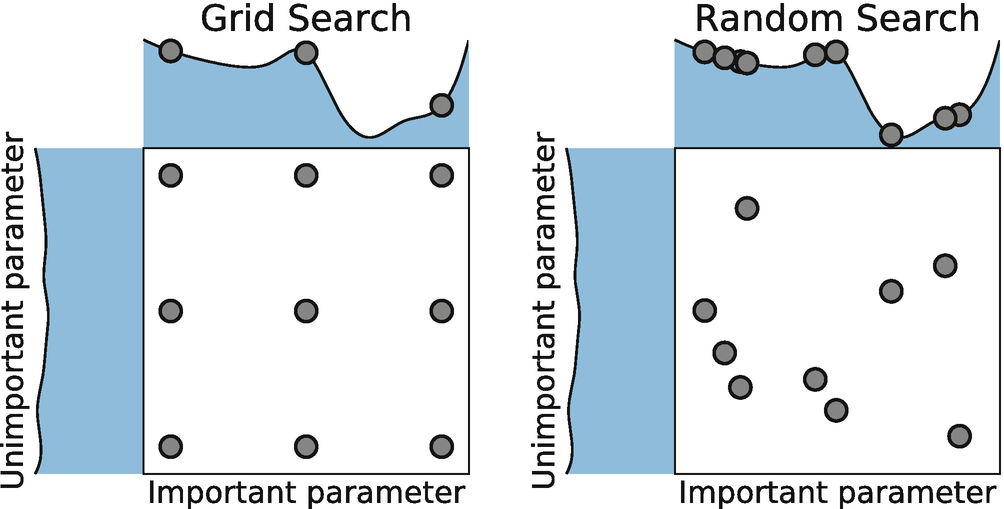
\includegraphics[width=.7\textwidth]{fig/L2/cIDuR2.png}
\end{figure}
\end{frame}

%%%%%%%%%%%%%%%%%%%%%%%%%%%%%%%%%%%%%%%%%%
\begin{frame}{Remarks on the random search procedure}

\begin{itemize}
    \item It \alert{does not make} an \alert{exhaustive} search of the hyperparameters
    \item The procedure is easy to \alert{parallelized}.
    \item The cost is predictable (number of draw).
\end{itemize}
\pause
Both gridsearch and random search are implemented and easy to use in scikit-learn.
\end{frame}


\begin{frame}{Bayesian search}
A more ''advance'' method it the \alert{Bayesian} optimization.\\
\vspace{1em}
The principle is to search hyperparameters where it is more likely to improve the model (based on previous attempts)\\
\vspace{1em}
Illustration taken from Ryan P. Adams: "A Tutorial on Bayesian Optimization for Machine Learning"
    
    
\end{frame}

\begin{frame}{}
    
\begin{figure}
        \centering
\multiinclude[<+->][format=png,graphics={width=\textwidth}]{fig/L2//hopt}  

    \end{figure}
    \rref[source: R.P. Adams]
    \end{frame}
%%%%%%%%%%%%%%%%%%%%%%%%%%%%%%%%%%%%%%%%%%
\section{Neural Networks}

\begin{frame}
  \frametitle{The perceptron : an artificial neuron}
  \begin{tikzpicture}[
    basic/.style={draw,fill=blue!20,text width=1em,text badly centered},
    input/.style={basic,circle},
    weights/.style={basic,rectangle},
functions/.style={basic,circle,fill=blue!10},
]
        \node[functions] (center) {};
        \node[below of=center,font=\scriptsize,text width=4em] {Activation function};
        \draw[thick] (0.5em,0.5em) -- (0,0.5em) -- (0,-0.5em) -- (-0.5em,-0.5em);
      %  \draw (0em,0.75em) -- (0em,-0.75em);
      %  \draw (0.75em,0em) -- (-0.75em,0em);
        \node[right of=center, anchor = west] (right) {$y=$ 0 ou 1};
            \path[draw,->] (center) -- (right);
        \node[functions,left=3em of center] (left) {$\sum$};
            \path[draw,->] (left) -- (center);
%        \node[weights,left=3em of left] (2) {$w_2$} -- (2) 
            \node[input,left= 4em of left] (l2) {$x_2$};
%            \path[draw,->] (l2) -- (2);
            \path[draw,->] (l2) -- node[above,midway]{$w_2$}(left);
        \node[below of=l2] (dots) {$\vdots$} ;
%(dots) node[left of=dots] (ldots) {$\vdots$};
%        \node[weights,below of=dots] (n) {$w_n$} -- (n) 
\node[input,below of=dots] (ln) {$x_n$};
%            \path[draw,->] (ln) -- (n);
            \path[draw,->] (ln) -- node[above,midway]{$w_n$}(left);
%        \node[weights,above of=2] (1) {$w_1$} -- (1) 
            \node[input,above of=l2] (l1) {$x_1$};
%            \path[draw,->] (l1) -- (1);
            \path[draw,->] (l1) -- node[above,midway]{$w_1$}(left);
%        \node[weights,above of=1] (0) {$w_0$} -- (0) 
\node[input,above of=l1] (l0) {$1$};
%            \path[draw,->] (l0) -- (0);
            \path[draw,->] (l0) -- node[above,midway]{$w_0$}(left);
        \node[below of=ln,font=\scriptsize](lin) {inputs};
        \node[right of=lin,xshift=+1em,font=\scriptsize] {weights};
    \end{tikzpicture}
\begin{block}{Computation}
$
y = f\left( w_0 + w_1. x_1 + w_2. x_2 +  \dots + w_n. x_n \right) = f\left( w_0 + \sum_{i=1}^n w_i.x_i\right)
$
\end{block}
\end{frame}

\begin{frame}{Some remarks}
\begin{itemize}[<+->]
    \item Inputs $x_i$ are the different features of the data
    \item Weight $w_i$ are the parameters of the model to optimize
    \item If the activation function is identity, it is equivalent to a linear regression
\end{itemize}
\visible<4->{
\begin{block}{}
More complexe models are build by combining several perceptrons
\end{block}
}

\end{frame}


\begin{frame}{Multi-layer perceptron (Densely connected layers)}
    \def\layersep{1.5cm}

\begin{tikzpicture}[
   shorten >=1pt,->,
   draw=black!50,
    node distance=\layersep,
    every pin edge/.style={<-,shorten <=1pt},
    neuron/.style={circle,fill=black!25,minimum size=17pt,inner sep=0pt},
    input neuron/.style={neuron, fill=green!50},
    output neuron/.style={neuron, fill=red!50},
    hidden neuron/.style={neuron, fill=blue!50},
    annot/.style={text width=4em, text centered}
]

    % Draw the input layer nodes
    \foreach \name / \y in {1,...,4}
    % This is the same as writing \foreach \name / \y in {1/1,2/2,3/3,4/4}
        \node[input neuron, pin=left:Feature \#\y] (I-\name) at (0,-\y) {};

    % set number of hidden layers
    \newcommand\Nhidden{3}

    % Draw the hidden layer nodes
    \foreach \N in {1,...,\Nhidden} {
       \foreach \y in {1,...,5} {
          \path[yshift=0.5cm]
              node[hidden neuron] (H\N-\y) at (\N*\layersep,-\y cm) {};
           }
    \node[annot,above of=H\N-1, node distance=1cm] (hl\N) {Hidden layer \N};
    }

    % Draw the output layer node
    \node[output neuron,pin={[pin edge={->}]right:Output}, right of=H\Nhidden-3] (O) {};

    % Connect every node in the input layer with every node in the
    % hidden layer.
    \foreach \source in {1,...,4}
        \foreach \dest in {1,...,5}
            \path (I-\source) edge (H1-\dest);

    % connect all hidden stuff
    \foreach [remember=\N as \lastN (initially 1)] \N in {2,...,\Nhidden}
       \foreach \source in {1,...,5}
           \foreach \dest in {1,...,5}
               \path (H\lastN-\source) edge (H\N-\dest);

    % Connect every node in the hidden layer with the output layer
    \foreach \source in {1,...,5}
        \path (H\Nhidden-\source) edge (O);

    % Annotate the layers

    \node[annot,left of=hl1] {Input layer};
    \node[annot,right of=hl\Nhidden] {Output layer};
\end{tikzpicture}
\end{frame}

\begin{frame}{Most usual activation functions}
\begin{columns}
\column{.5\textwidth}
    \begin{figure}
        \centering
        Linear\\
        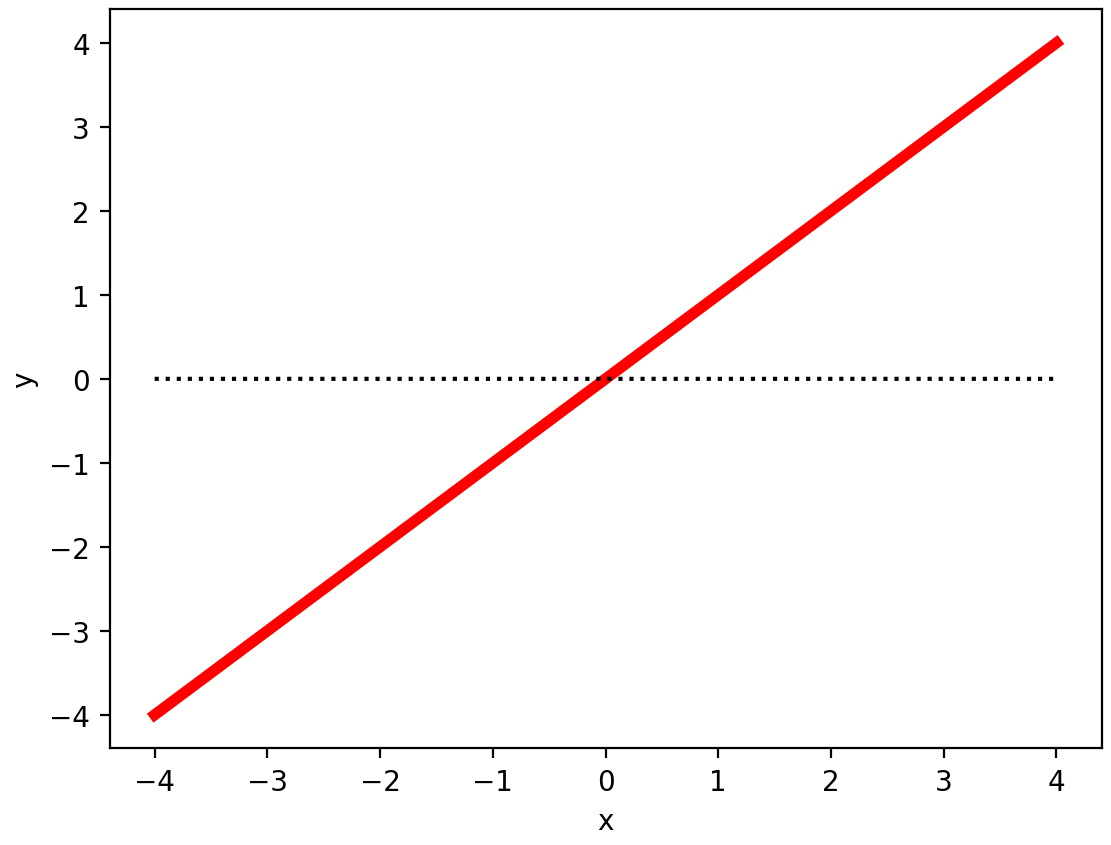
\includegraphics[width=.85\textwidth]{fig/L2/activ-linear.png}\\
        ReLU\\
        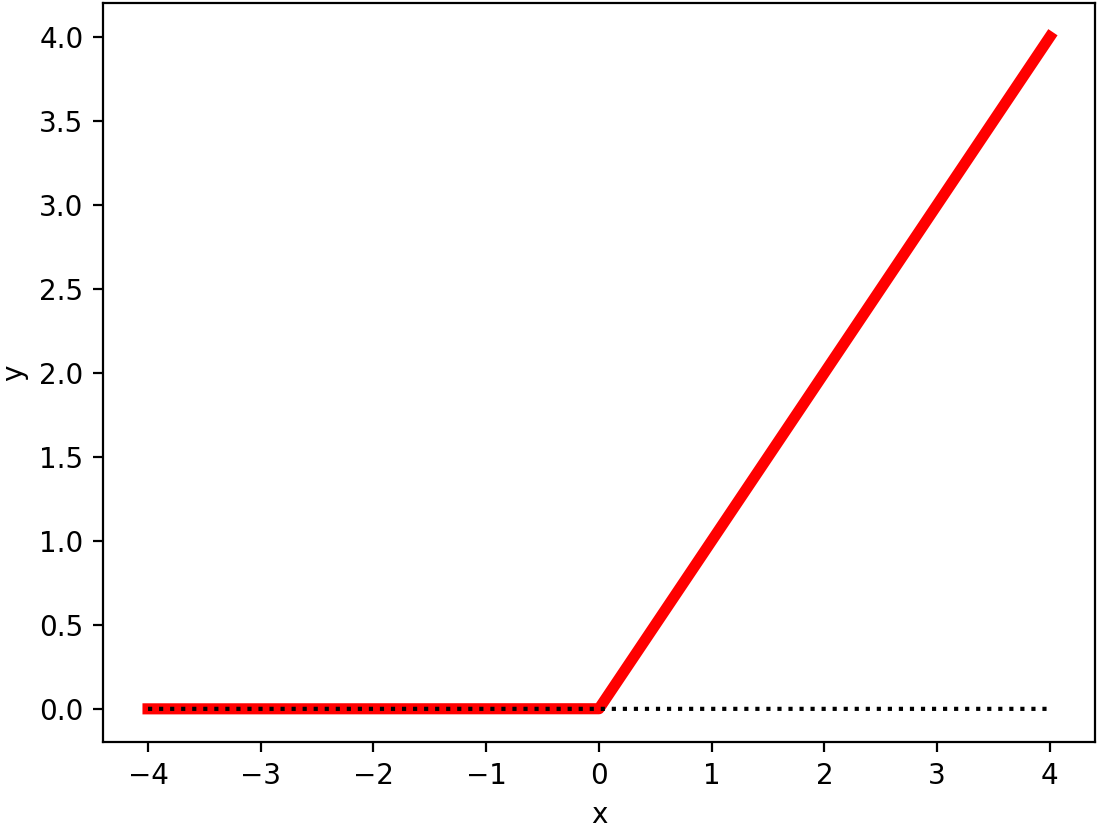
\includegraphics[width=.85\textwidth]{fig/L2/activ-relu.png}\\

    \end{figure}
\column{.5\textwidth}
    \begin{figure}
     \centering
        Hyperbolic tangent\\
        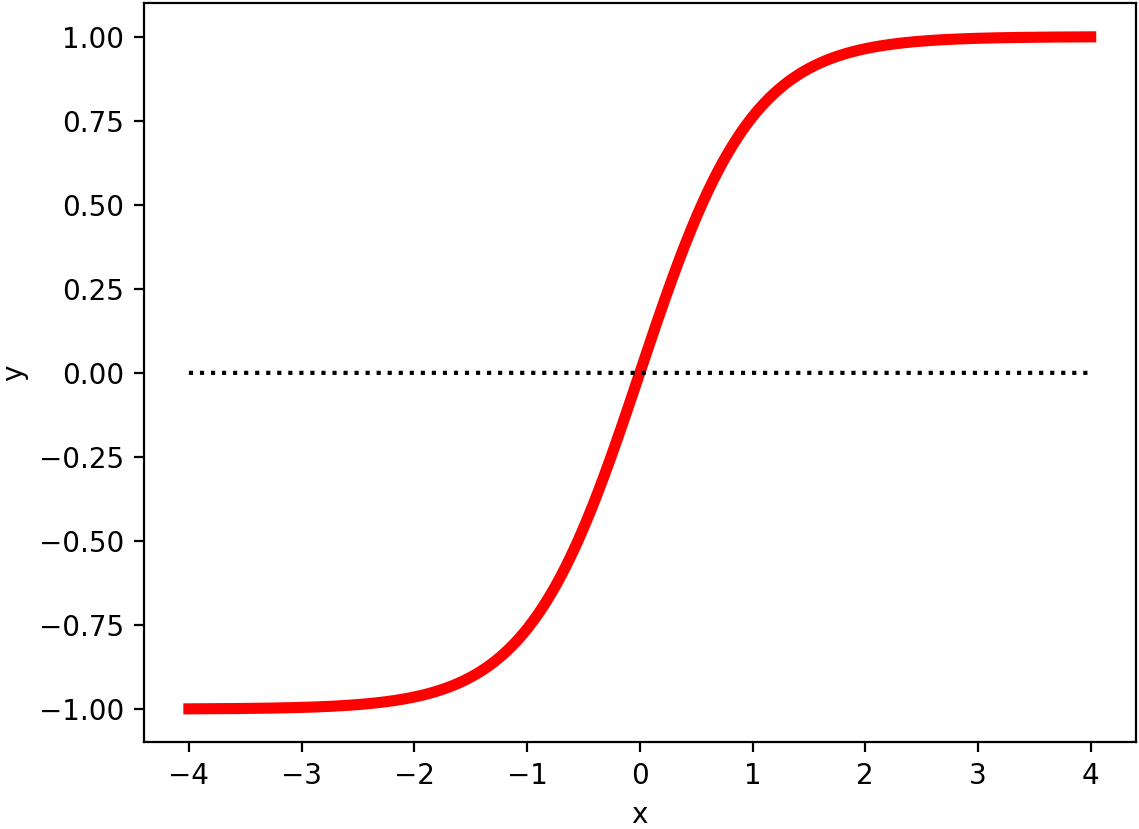
\includegraphics[width=.85\textwidth]{fig/L2/activ-tanh.png}\\
       Sigmoid\\
        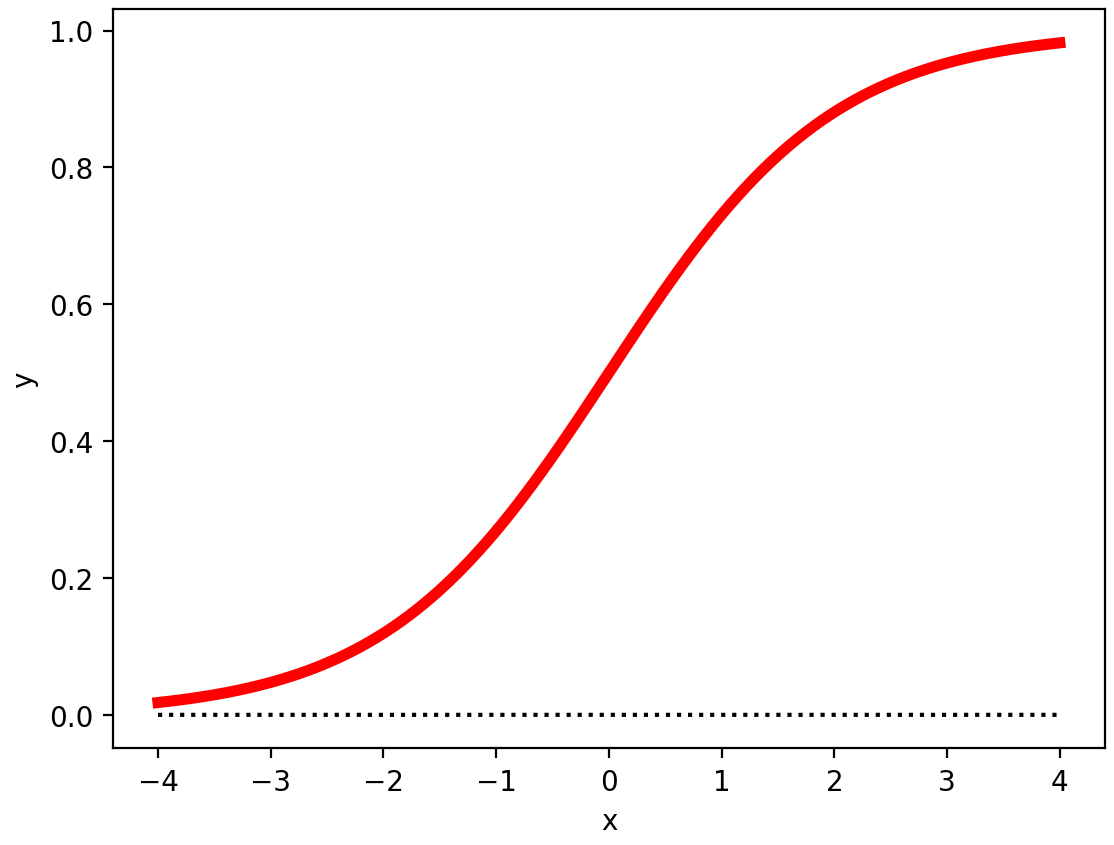
\includegraphics[width=.85\textwidth]{fig/L2/activ-sigmoid.png}\\

    \end{figure}
\end{columns}
\end{frame}


\begin{frame}{New fancy activation functions}
\begin{columns}
\column{.5\textwidth}
    \begin{figure}
        \centering
        Leaky-ReLU\\
        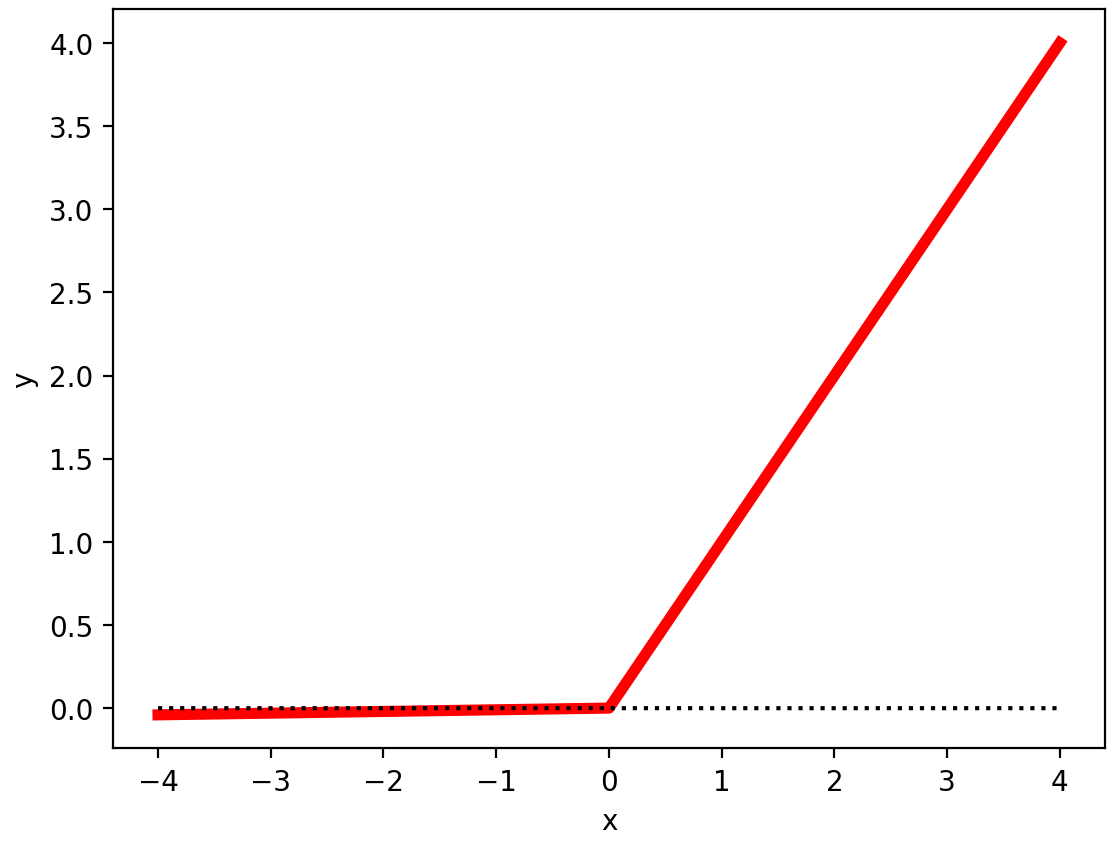
\includegraphics[width=.85\textwidth]{fig/L2/activ-l-relu.png}\\
      

    \end{figure}
\column{.5\textwidth}
    \begin{figure}
     \centering
        Swish\\
        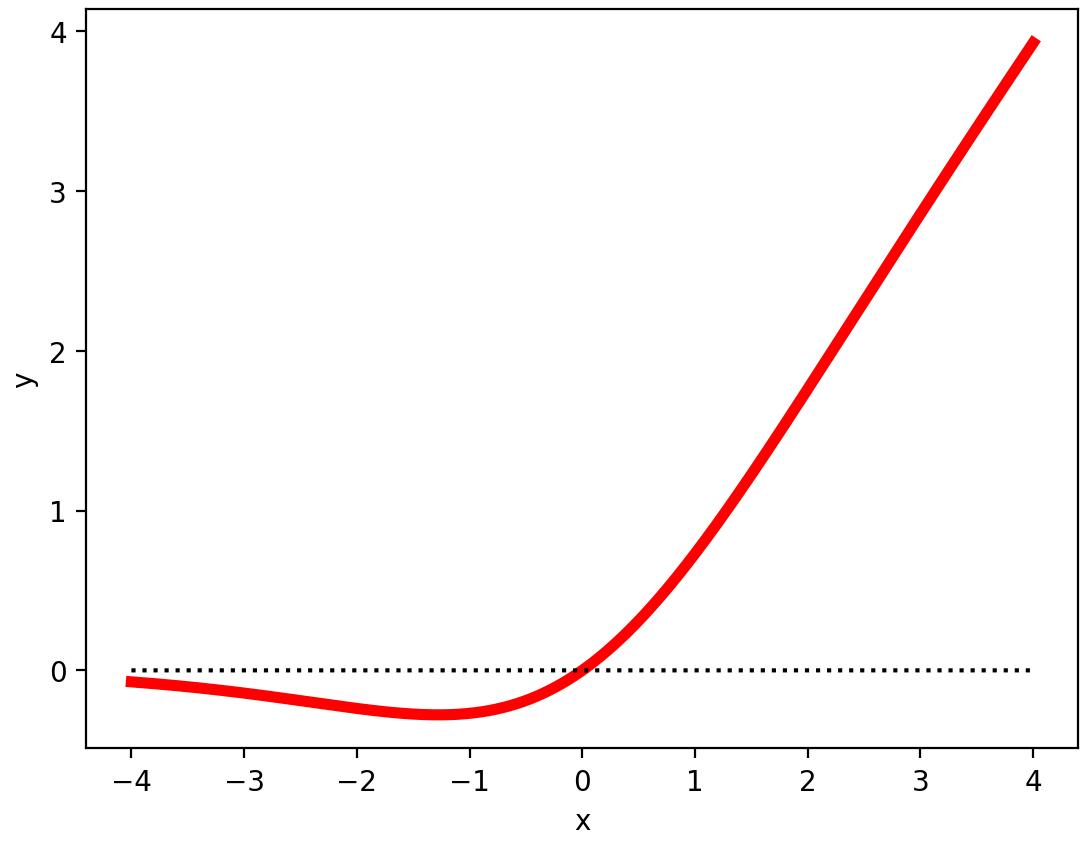
\includegraphics[width=.85\textwidth]{fig/L2/activ-swish.png}\\
     

    \end{figure}
\end{columns}
\end{frame}


\begin{frame}{Classification and regression loss}
  
   \begin{columns}
   \column{.5\textwidth}
   \alert{Regression}
   \begin{itemize}
       \item Last layer:\\
       linear or hyperbolic tangent
       \item Loss function:\\
       $$L(\hat{y},y) = \sum_i (\hat{y}_i-y_i)^2$$
   \end{itemize}
   \pause
\column{.5\textwidth}
       \alert{Classification}
   \begin{itemize}
       \item Last layer:\\
       Soft-max
       $$
       p_j=f_j(\mathbf{h}) = \frac{e^{h_j}}{\sum_k e^{h_k}}
       $$
       
       \item Loss function:\\
       Negative crossentropy
       $$L(p,y) = -\sum_i \sum_j y_{i,j}.\log{p_{i,j}}$$
   \end{itemize}
   \end{columns}
\end{frame}

\begin{frame}{Classification loss (binary case)}
Objective: binary classification (the model determine if the input feature is in a class or not)\\
\vspace{1em}

Exemple: Try to know if an image is a cat or not.\\
\vspace{1em}

Dataset:

\begin{table}[]
    \centering
    \begin{tabular}{ccccc}
        {\bf x (feature)} &
         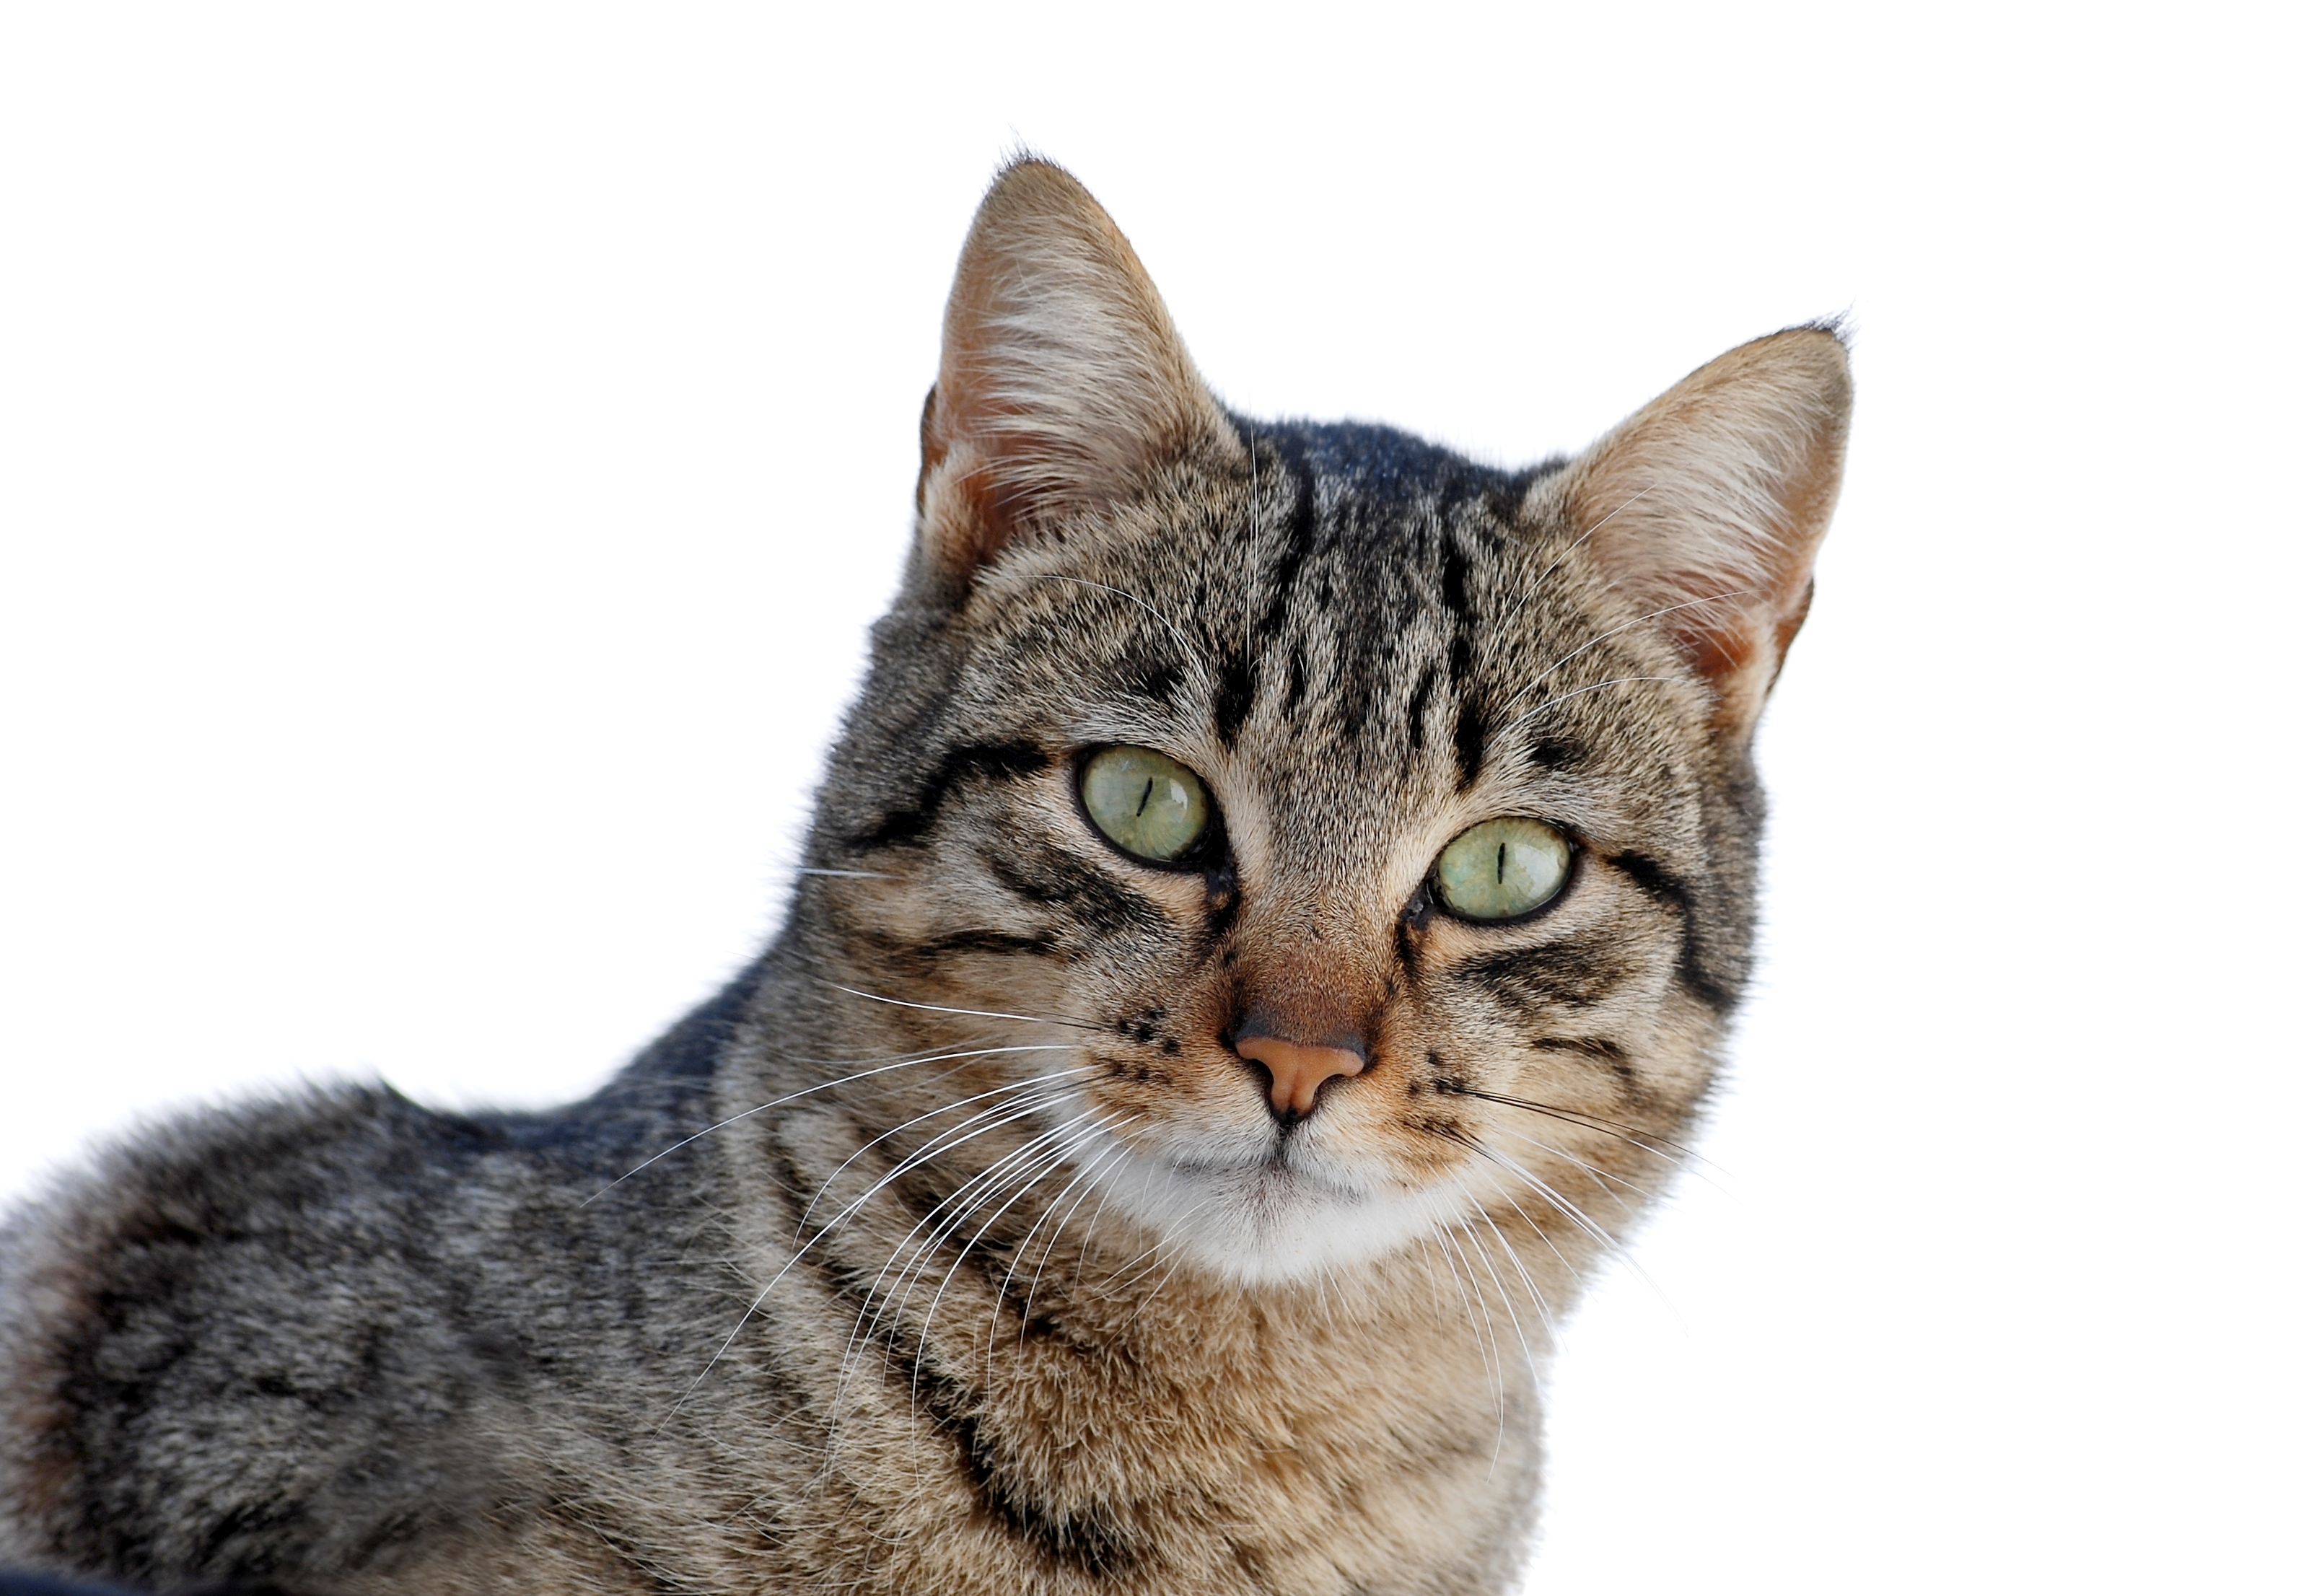
\includegraphics[width=.2\textwidth]{fig/L2/cat1.jpg}& 
         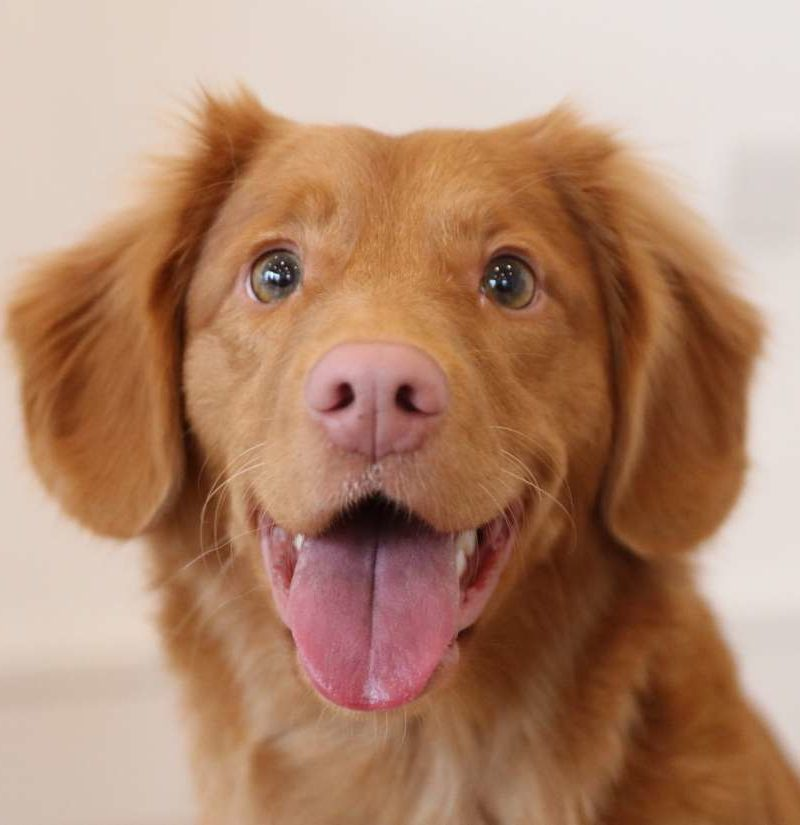
\includegraphics[width=.2\textwidth]{fig/L2/dog1.jpg}&
         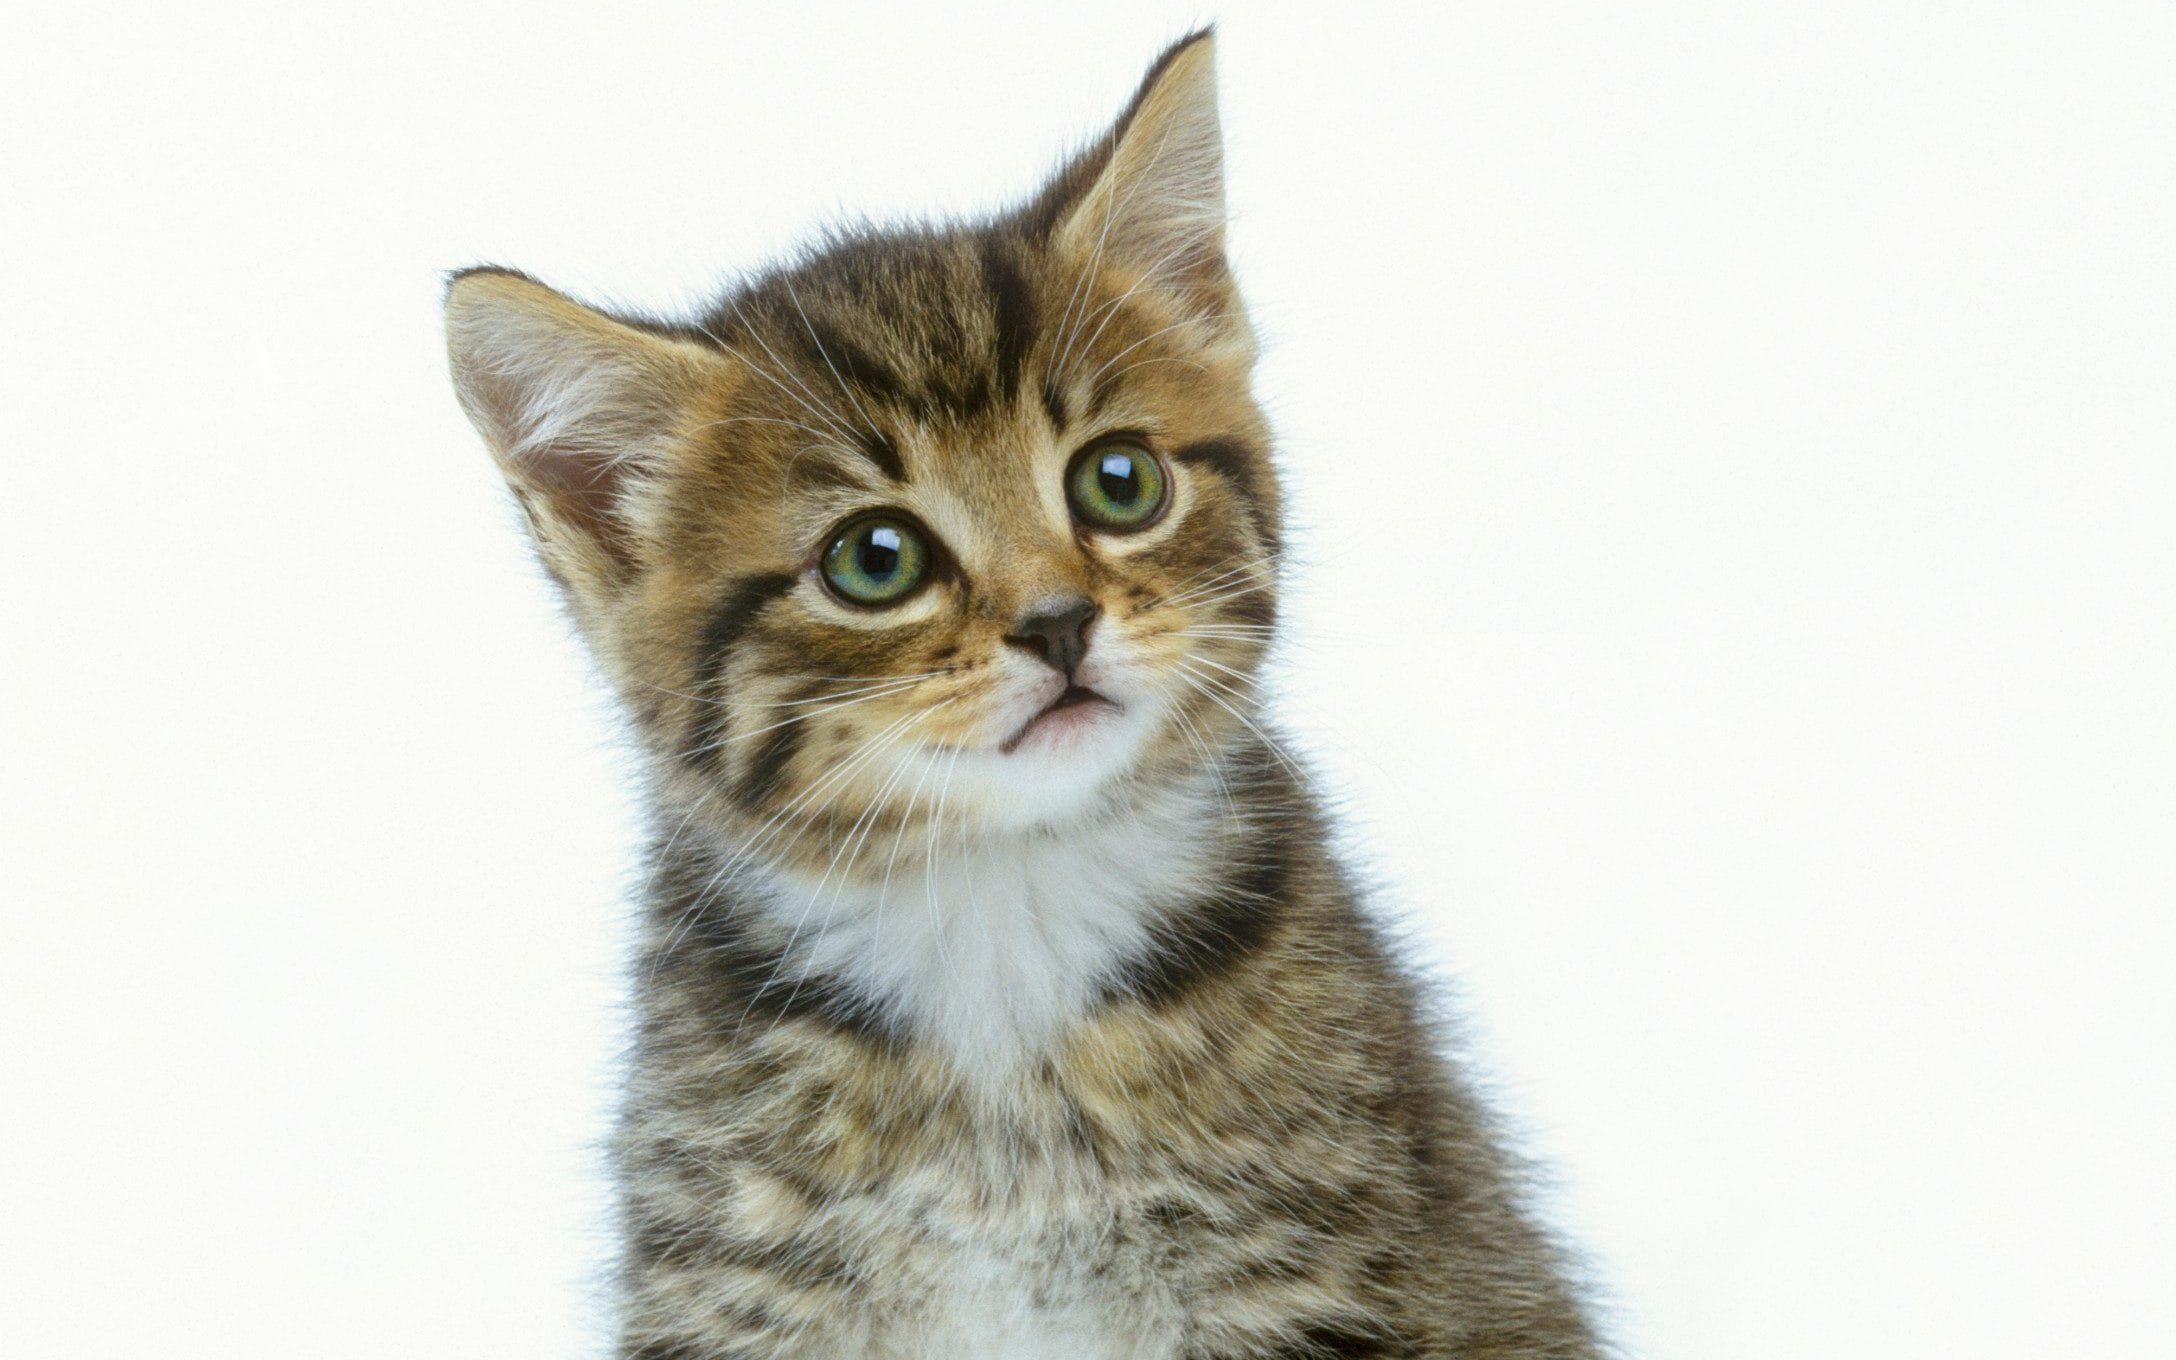
\includegraphics[width=.2\textwidth]{fig/L2/cat2.jpg}&
         ...
         \\
        {\bf y (target)} & Cat & Dog & Cat & ...\\
    \end{tabular}
\end{table}

\end{frame}

\begin{frame}{How to proceed?}

\begin{enumerate}[<+->]
    \item Encode the targets (1 for cat, 0 otherwise)
    \begin{table}[]
    \centering
    \begin{tabular}{ccccc}
    
        {\bf y (target)} & Cat & Dog & Cat & ...\\
         {\bf y (encoded)} & 1 & 0 & 1 & ...\\
        
    \end{tabular}
\end{table}
    \item Design a model with \alert{\bf one output } and use the \alert{\bf sigmoid} as output activation function of your model $f(x)$, so $0 < f(x) < 1$.\\
    Rule: if $f(x)>\frac{1}{2}$, classify as ''Cat''.\\
    \alert{\bf f(x) is interpreted as the probability of the image x to be a cat.}
    \item Loss function to minimize is binary cross entropy:
    $$
    L = -\sum y_i \cdot \log(f(x_i)) + (1-y_i)\cdot \log (1-f(x_i))
    $$
\end{enumerate}    
\end{frame}

\begin{frame}{Classification loss (multiclass)}
Objective:  classification (the model determine in which class the input feature (more than 2 classes))\\
\vspace{1em}

Exemple: Try to know if an image is a cat, a dog or a duck.\\
\vspace{1em}

Dataset:

\begin{table}[]
    \centering
    \begin{tabular}{ccccc}
        {\bf x (feature)} &
         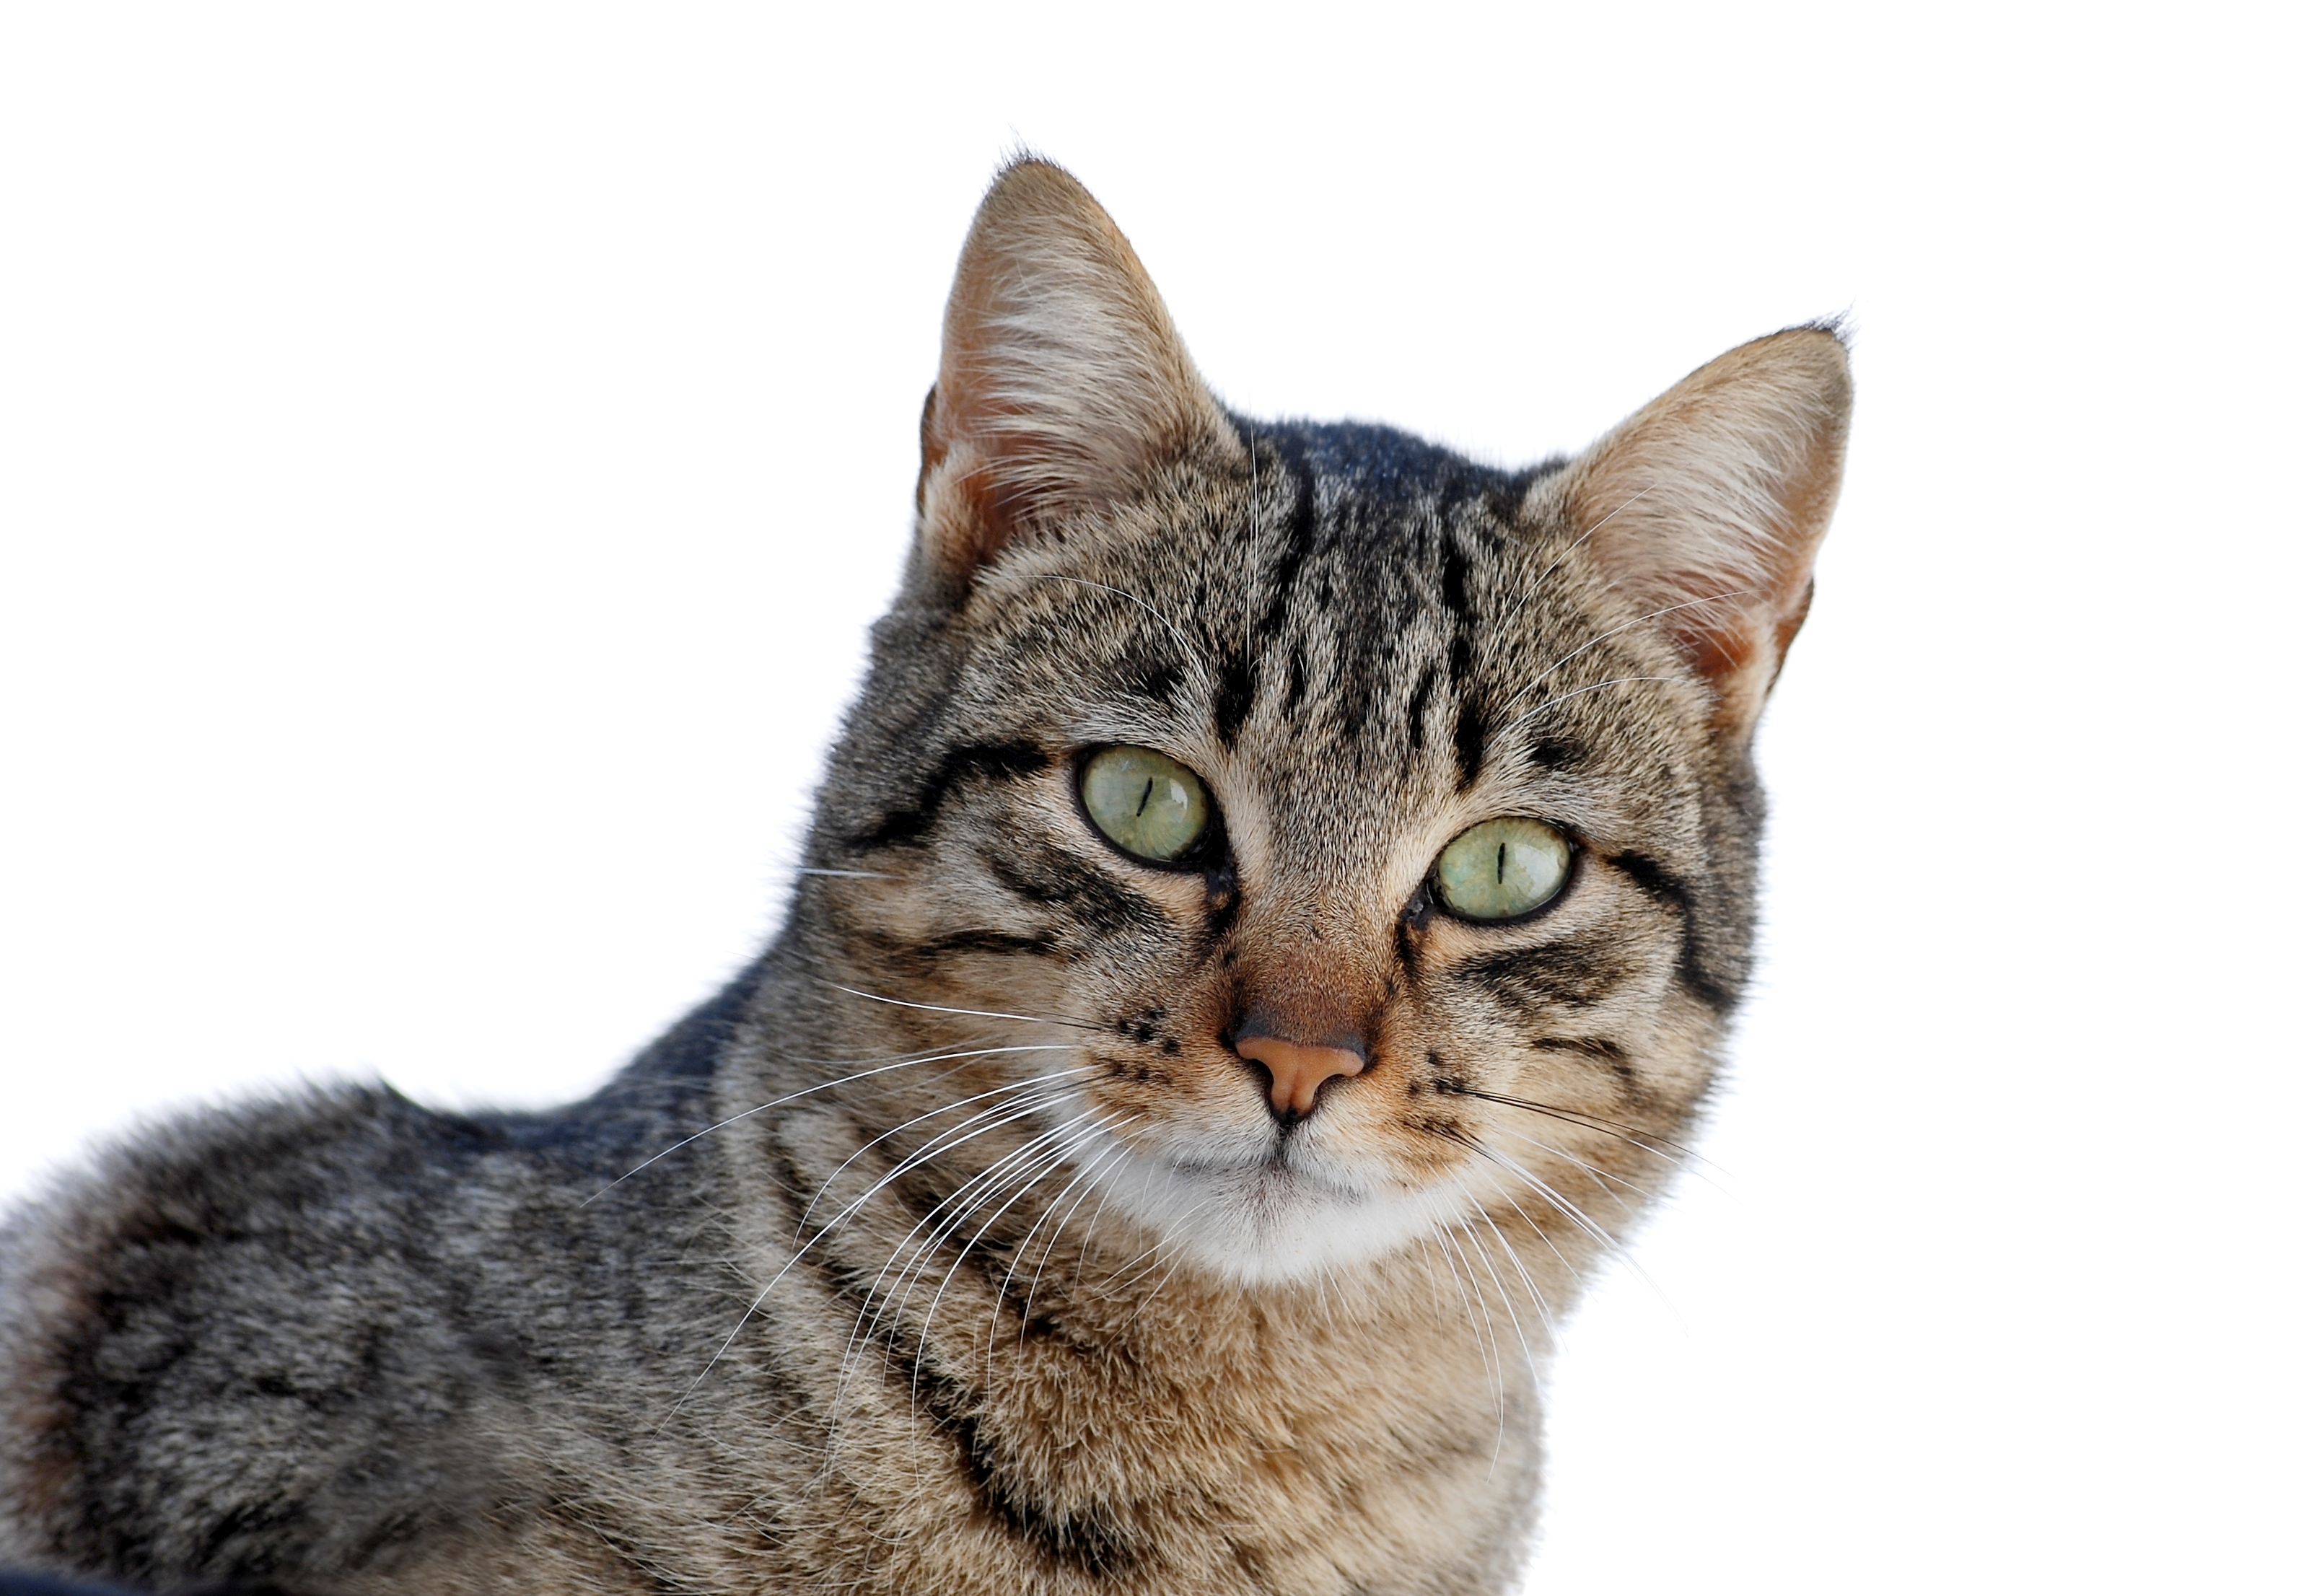
\includegraphics[width=.2\textwidth]{fig/L2/cat1.jpg}& 
         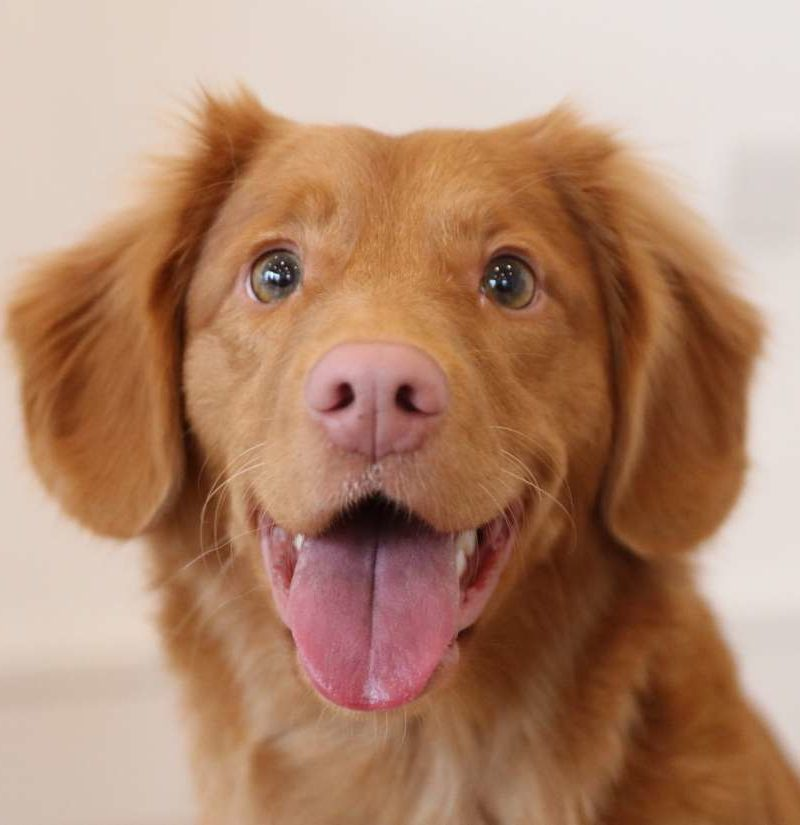
\includegraphics[width=.2\textwidth]{fig/L2/dog1.jpg}&
         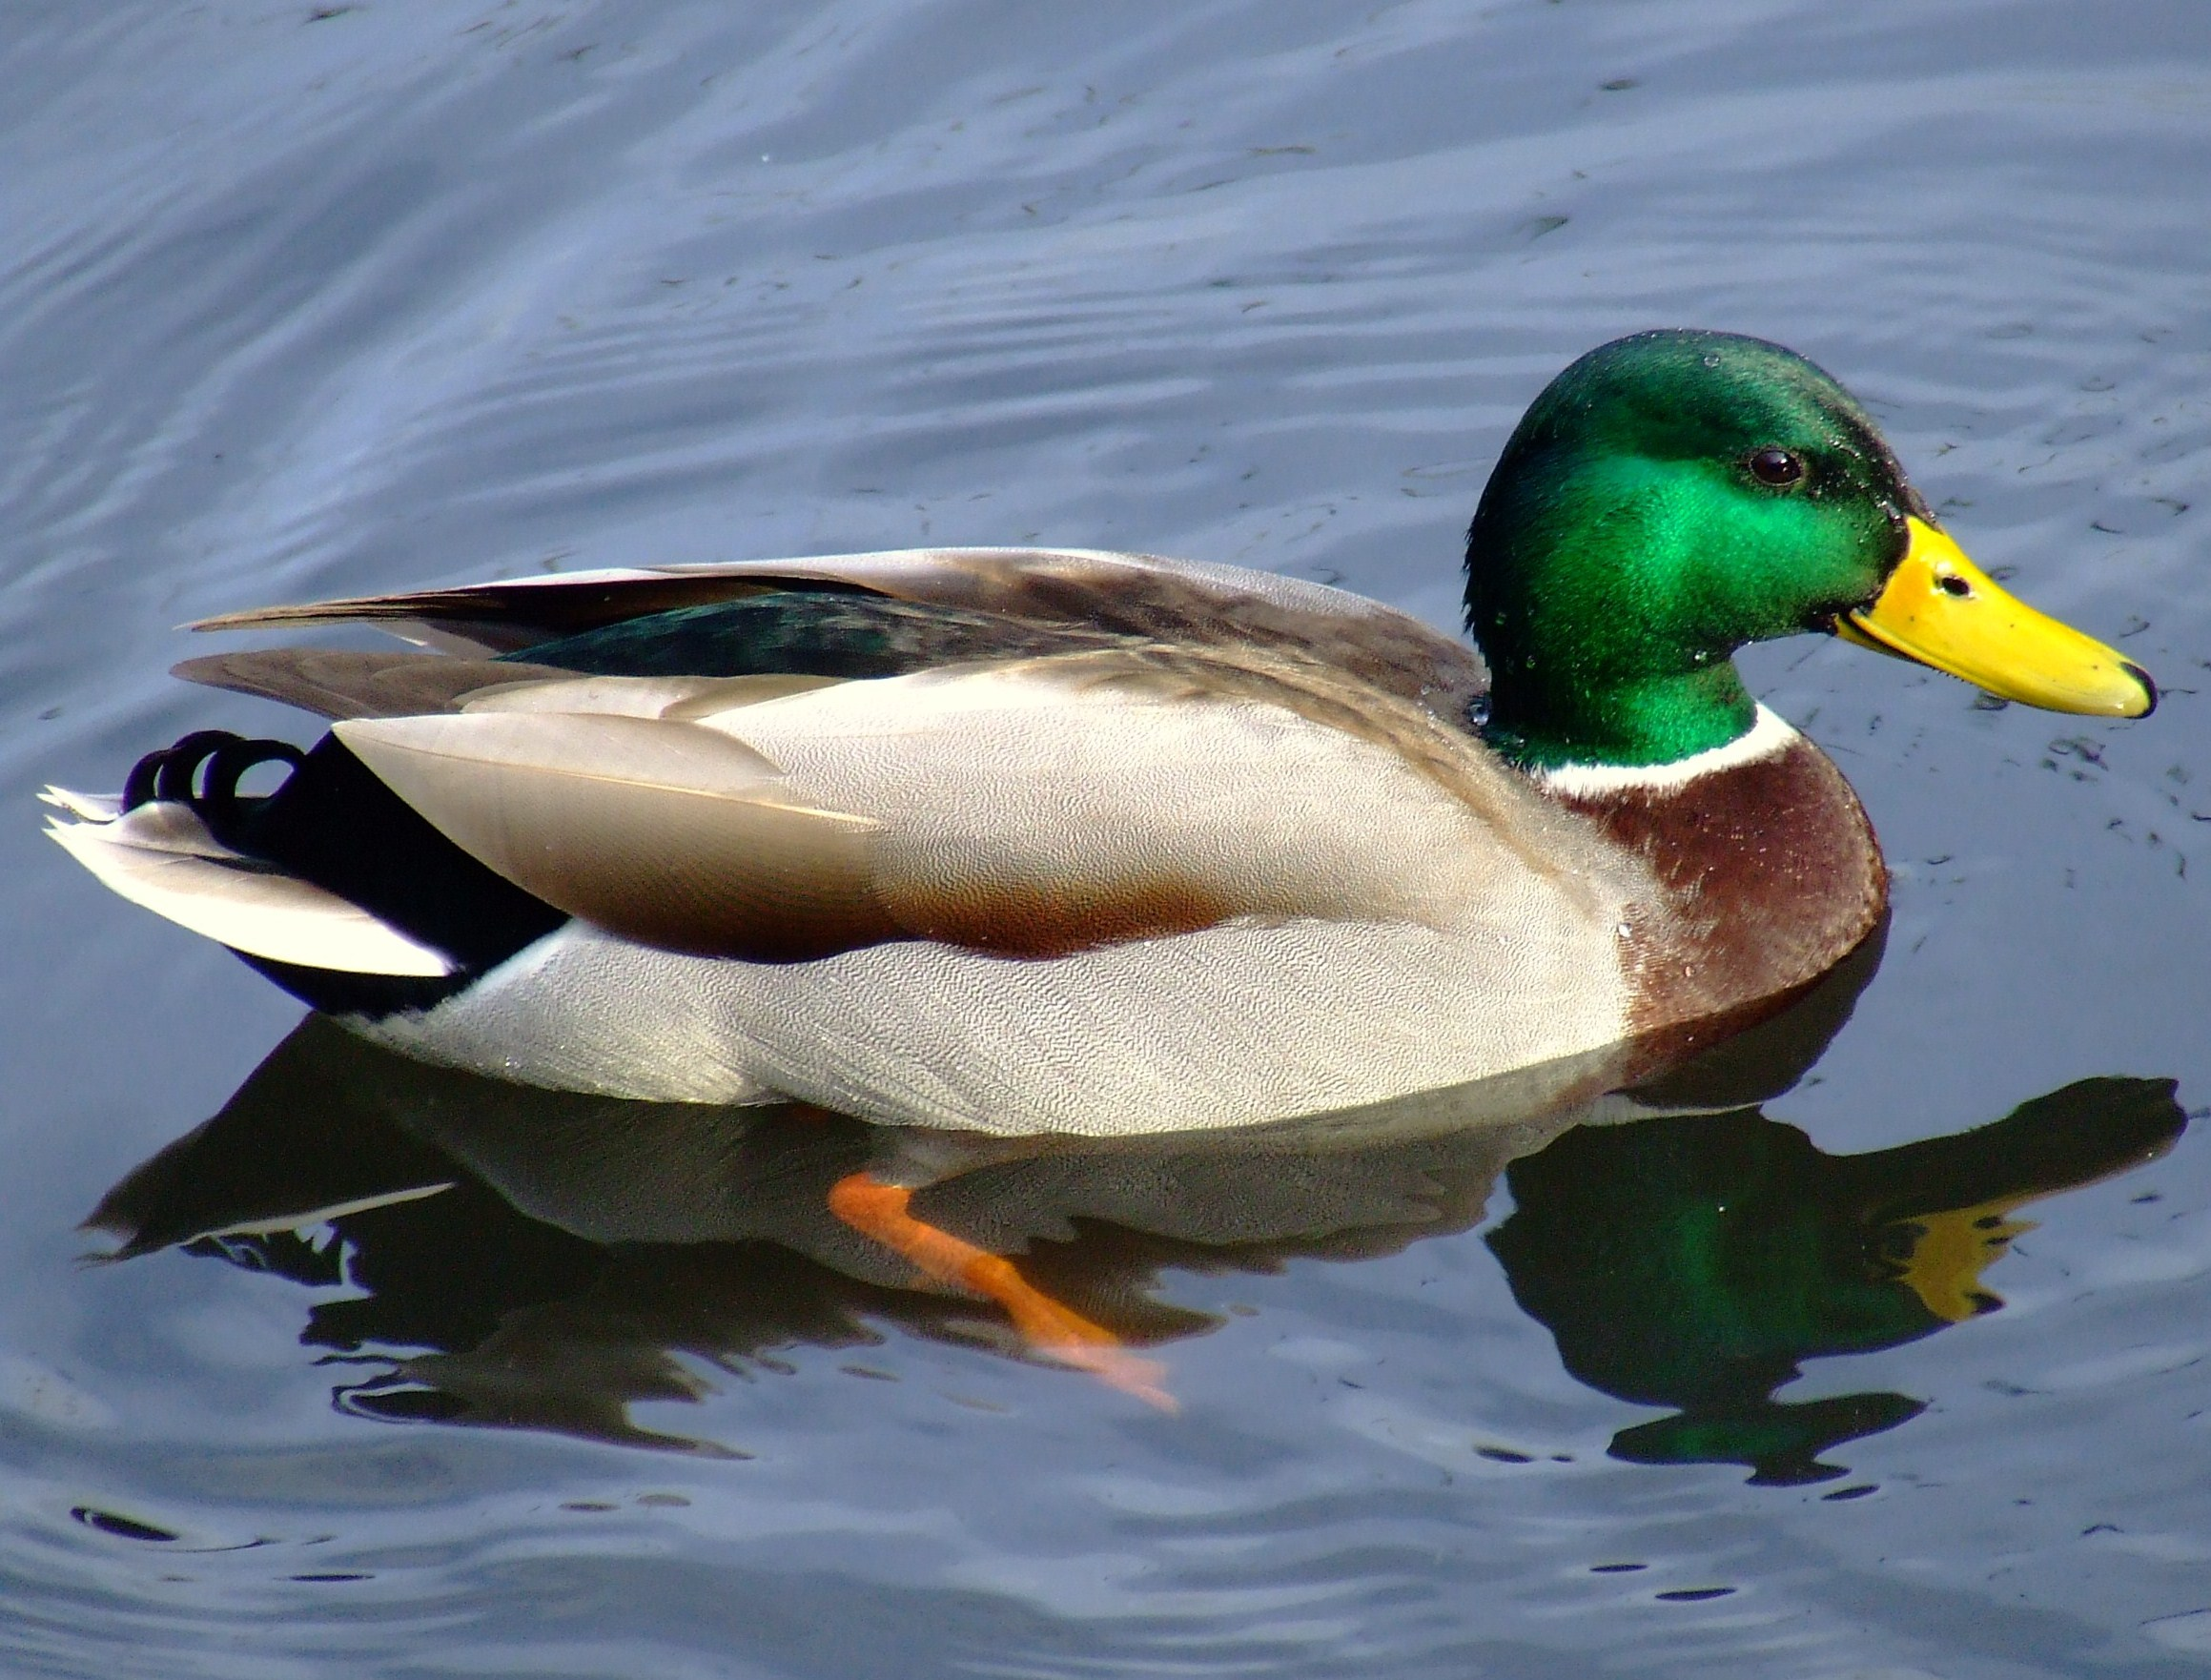
\includegraphics[width=.2\textwidth]{fig/L2/duck1.jpg}&
         ...
         \\
        {\bf y (target)} & Cat & Dog & Duck & ...\\
    \end{tabular}
\end{table}

\end{frame}

\begin{frame}{How to proceed?}

\begin{enumerate}[<+->]
    \item Encode the targets using one hot encoding
    \begin{table}[]
    \centering
    \begin{tabular}{ccccc}
    
        {\bf y (target)} & Cat & Dog & Cat & ...\\
         {\bf y (encoded)} & $(1,0,0)$ & $(0,1,0)$ & $(0,0,1)$ & ...\\
        
    \end{tabular}
\end{table}
    \item Design a model with \alert{\bf $N$ outputs } ($N$ being the number of modalities) and use the \alert{\bf soft-max} as output activation function
    $$
       p_j=f_j(\mathbf{h}) = \frac{e^{h_j}}{\sum_k e^{h_k}}
    $$
    Rule: the class is attributed to the argument of the maximum of ${\bf p}$. Ex ${\bf p} = (0.1, 0,7, 0,2)$ is classified as ''dog''.
    \alert{\bf $p_j$ is interpreted as the probability of the image x to belong to the class $j$}
    \item Loss function to minimize is negative cross entropy
 $$L = -\sum_i \sum_j y_{i,j}.\log{p_{i,j}}$$
\end{enumerate}    
\end{frame}


\begin{frame}[fragile]{Convolutional neural net}
    \begin{tikzpicture}
    \draw[step=0.8,color=gray] (0,0) grid (4.8,4.8);
    \matrix[matrix of nodes,
    inner sep=0pt,
    anchor=south west,
    nodes={inner sep=0pt,text width=.8cm,align=center,minimum height=0.8cm}
    ]{
    $x_{11}$ & $x_{12}$ & $x_{13}$& $x_{14}$ & $x_{15}$  & $x_{16}$ \\
     $x_{21}$ & $x_{22}$ & $x_{23}$& $x_{24}$ & $x_{25}$ &  $x_{26}$ \\
    $x_{31}$ &$x_{32}$ & $x_{33}$& $x_{34}$ & $x_{35}$  & $x_{36}$ \\
    $x_{41}$ &$x_{42}$ & $x_{43}$& $x_{44}$ & $x_{45}$ & $x_{46}$  \\
     $x_{51}$ &$x_{52}$ & $x_{53}$& $x_{54}$ & $x_{55}$&  $x_{56}$  \\
     $x_{61}$ &$x_{62}$ & $x_{63}$& $x_{64}$ & $x_{65}$&  $x_{66}$  \\
    };
    \node (in) at (4.8,2.4) {} ;
    \node (out) at (8,2.4) {} ;
    \draw[step=0.8,color=gray] (8,0.8) grid (11.2,4);
    \matrix[matrix of nodes,
    xshift=8cm,
    yshift=0.8cm,
    inner sep=0pt,
    anchor=south west,
    nodes={inner sep=0pt,text width=.8cm,align=center,minimum height=0.8cm}
    ]{
    $h_{11}$ & $h_{12}$ & $h_{13}$& $h_{14}$ \\
     $h_{21}$ & $h_{22}$ & $h_{23}$& $h_{24}$ \\
    $h_{31}$ &$h_{32}$ & $h_{33}$& $h_{34}$   \\
    $h_{41}$ &$h_{42}$ & $h_{43}$& $h_{44}$  \\
    };
    
    \draw[step=0.5,color=gray] (5.999,3.499) grid (7.5,5);
    \matrix[matrix of nodes,
    xshift=5.999cm,
    yshift=3.499cm,
    inner sep=0pt,
    anchor=south west,
    nodes={inner sep=0pt,fill=orange!20,font=\footnotesize,text width=.5cm,align=center,minimum height=0.5cm}
    ]{
    $w_{11}$ & $w_{12}$ & $w_{13}$ \\
    $w_{21}$ & $w_{22}$ & $w_{23}$ \\
    $w_{31}$ & $w_{32}$ & $w_{33}$ \\
    };
    
    \path [draw, very thick, ->] (in) edge[bend left=40] 
    node [above,midway]{$\mathbf{w}$}(out);
    \node (xlabel) at (2.4,5) {$X$: an image};
    \node (hlabel) at (9.6,4.2) {$h$: first feature};
    \end{tikzpicture}
    \begin{block}{Perform a standard convolution}
    $$
    h_{i,j} = \sum_{k=1}^3\sum_{l=1}^3 x_{i+k-1,j+l-1}.w_{k,l}
    $$
    \end{block}
\end{frame}


\begin{frame}[t]{Main parameters of a convolutional layer}
\begin{itemize}
    \item <1-> \alert<1> {Size of the filter} $K$ 
    \item <2-> \alert<2> {Number of filters} $p$

\only<2>{
A convolutional layer is composed of $p$ convolutions (size of layer) extracting $p$ features from the data.
\begin{figure}
\centering
    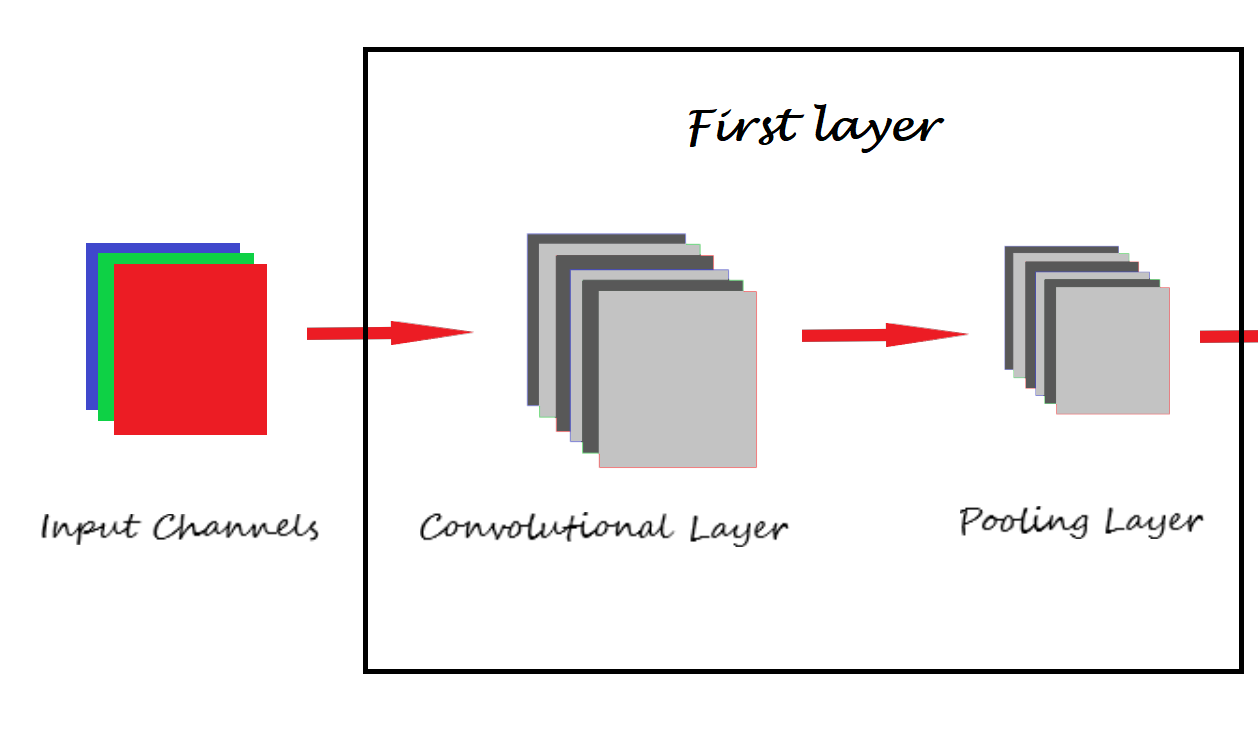
\includegraphics[width=.6\textwidth,trim={0 3.5cm 12.5cm 5cm},clip]{fig/L2/Cnn-layer.png}
\end{figure}
}

    \item <3-> \alert<3> {Strides} $S$
    
    \only<3> {
{\centering
\begin{tabular}{cc}
    $S=1$ & $S=2$ \\
    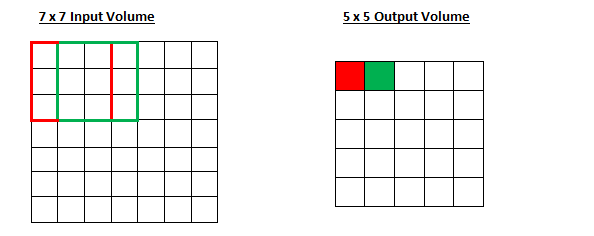
\includegraphics[trim={0.5cm 0 2.5cm 0}, clip, width=.5\textwidth]{fig/L2/Stride1.png}&
    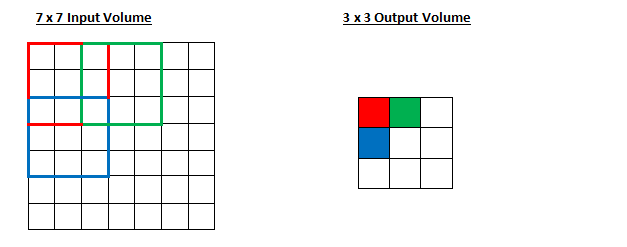
\includegraphics[trim={0 0 2.5cm 0}, clip, width=.5\textwidth]{fig/L2/Stride2.png}\\
    \end{tabular}
    }}
    
    \item <4-> \alert<4> {Padding} $P$
    
    {\only<4>
    {\centering
\begin{tabular}{cc}
    $P=1$ & $P=2$ \\
    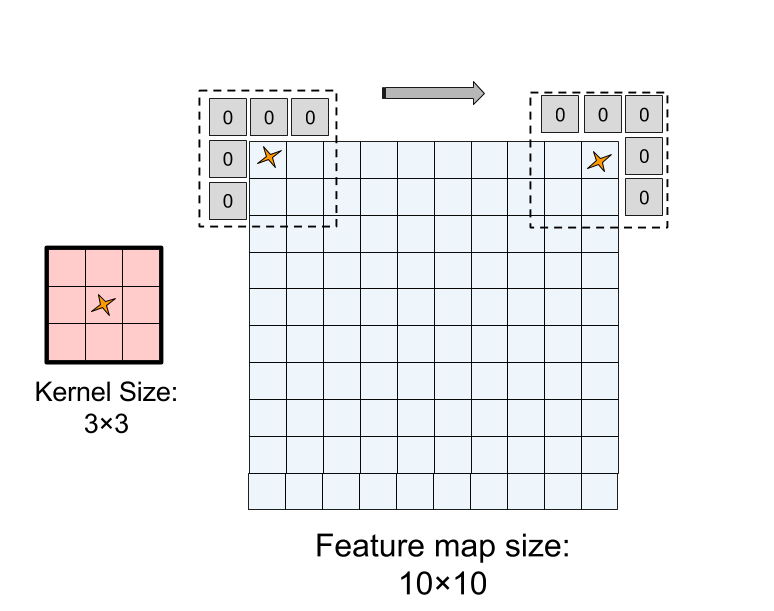
\includegraphics[trim={0 0 1.5cm 0}, clip, width=.45\textwidth]{fig/L2/pad3.png}&
    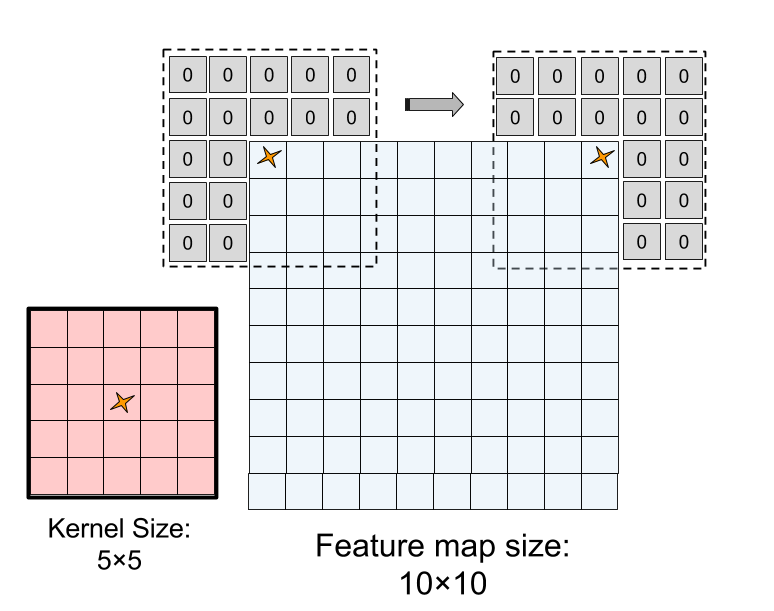
\includegraphics[trim={0 0 1.5cm 0}, clip, width=.45\textwidth]{fig/L2/pad5.png}\\
    \end{tabular}
    }

}
    
\end{itemize}
    \pause
    {\footnotesize
    $O = \frac{W - K +2P}{S} + 1$, where $O$ is the output size and $W$ the input size.
    }
\end{frame}


\begin{frame}{Summary of Convolutional layer steps}
    \begin{figure}
        \centering
        1. Convolution
\multiinclude[<+->][format=png,graphics={width=\textwidth}]{fig/L2/animated/conv}       
    \end{figure}
    \pause
    \vspace{-2em}
    \begin{columns}[t]
    \column{.7\textwidth}
    \begin{figure}
        \centering
        2. Addition
            \multiinclude[<+->][format=png,graphics={width=\textwidth}]{fig/L2/animated/channels}       

    \end{figure}
    
       \column{.3\textwidth}
       \pause
    \begin{figure}
        \centering
        3. Bias\\
\multiinclude[<+->][format=png,graphics={width=.6\textwidth}]{fig/L2/animated/bias}       
    \end{figure}
    \end{columns}
\end{frame}

\begin{frame}{Remarks on Convolutional layers}
\begin{itemize}
    \item Convolutional layers are acting locally on the image (But you can still use large scale information by adding more layers)
    \item Convolutions are invariant by translation (the weights do not depend on the location on the image).
    \item They can handle images of different sizes.
    
\end{itemize}
    
\end{frame}
\begin{frame}{Max-Pooling}
    In order to reduce the size of the feature space (en to enhance the gradients), a common operation is to perform a max-pooling.
    \begin{figure}
   \centering
    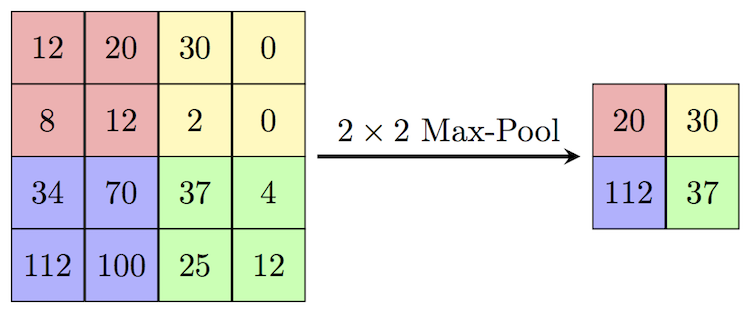
\includegraphics[width=.6\textwidth]{fig/L2/MaxpoolSample2.png}
\end{figure}
\end{frame}

\begin{frame}[fragile]{A traditionnal CNN architecture}
    \begin{figure}
\centering
    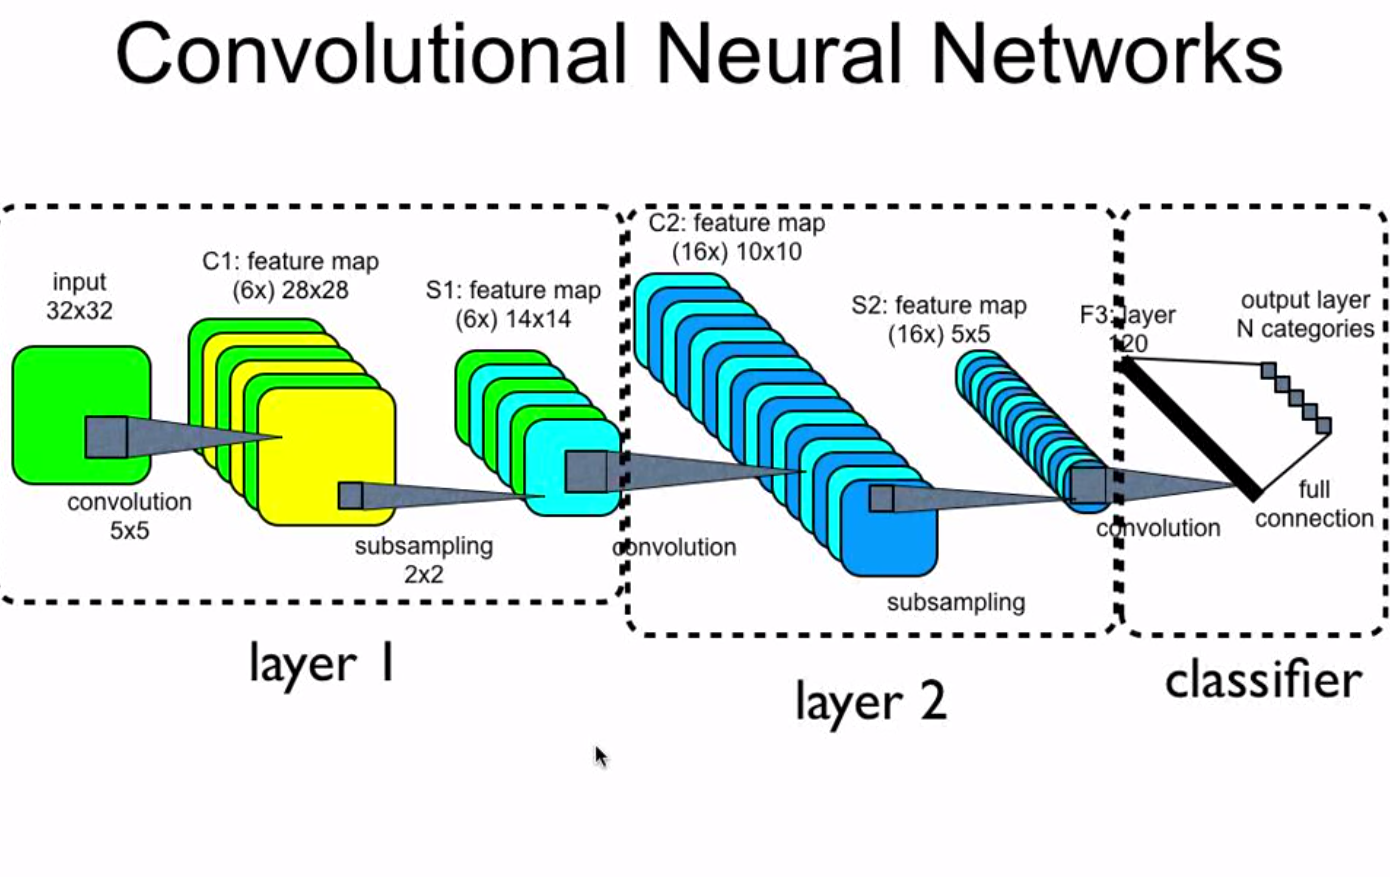
\includegraphics[width=.8\textwidth,trim={0 0cm 0cm 3cm},clip]{fig/L2/CNN.png}
\end{figure}
\end{frame}

\begin{frame}{Example of AlexNet}
    \alert{AlexNet} is the first Deep architecture used on ImageNet challenge in 2012 and achieved an \alert{error of 15.3\%} (10\% better than the previous best classifier). The paper was cited more than 34,000 times.

\begin{thebibliography}{GBC16}

\bibitem[KH12]{Krizhevsky2012ImageNetNetworks}
Alex Krizhevsky and Geoffrey~E Hinton, \emph{{ImageNet Classification with Deep
  Convolutional Neural Networks}}, Neural Information Processing Systems
  (2012), 1--9.

\end{thebibliography}
    \begin{figure}
        \centering
        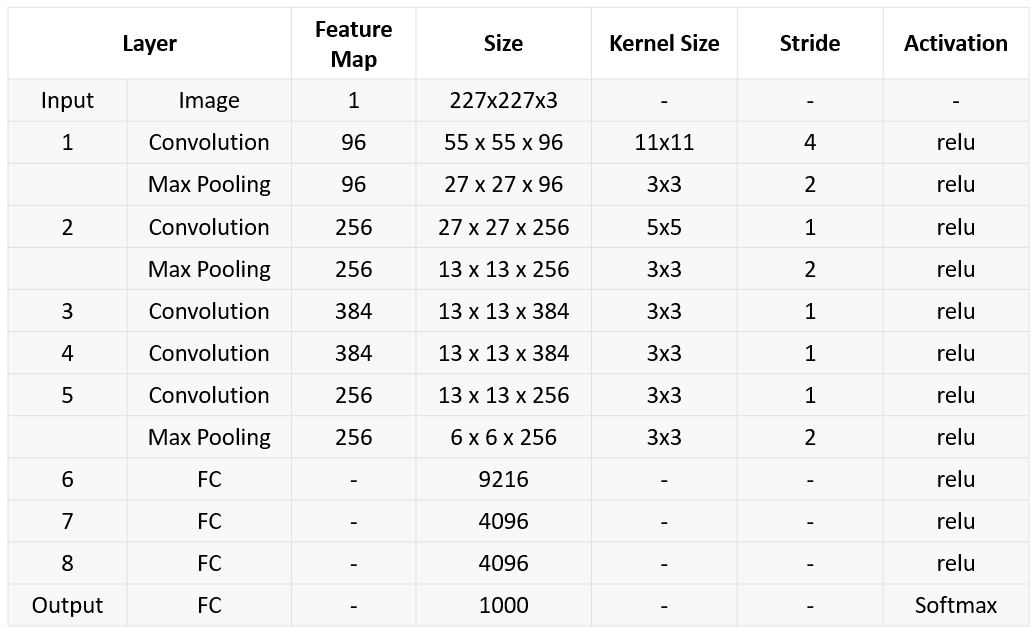
\includegraphics[width=.5\textwidth]{fig/L2/AlexNet_Summary_Table.jpg}

    \end{figure}
\end{frame}


\section{Optimization using gradient descent}
\begin{frame}{What is gradient descent}
\begin{block}{Objective}
Minimize the function $L(\boldsymbol{\theta})$ where $\boldsymbol{\theta}$ is a vector of parameters (e.g. weights of a neural net).
\end{block}
Example with $\boldsymbol{\theta} = (w, b)$
\begin{columns}

\column{.5\textwidth}
\begin{figure}
    \centering
    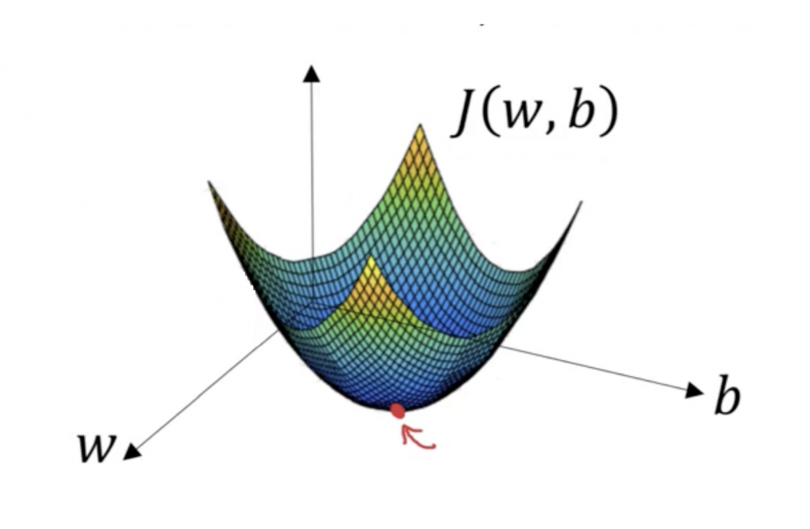
\includegraphics[width=.9\textwidth]{fig/L3/gradient-descent-convex-function.png}
\end{figure}

\column{.5\textwidth}
\begin{figure}
    \centering
    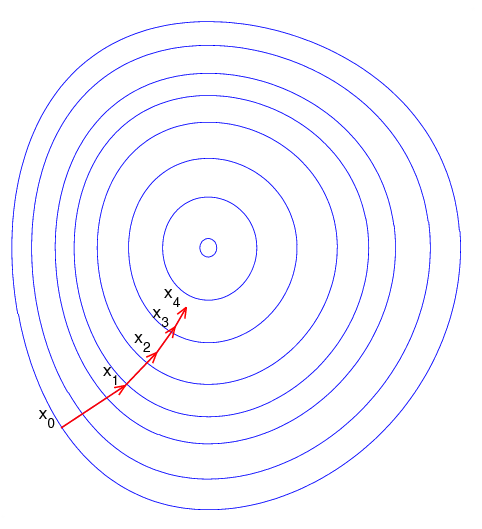
\includegraphics[width=.8\textwidth]{fig/L3/gradient-descent-range.png}
\end{figure}
\end{columns}

\end{frame}
 \begin{frame}{Iterative algorithm}
  \begin{enumerate}[<+->]
      \item We start with a "first guess" of the parameter $\boldsymbol{\theta}_0$
      \item we iterate over several values of the parameters following the update rule:
      $$
      \boldsymbol{\theta}_{k+1} = \boldsymbol{\theta}_{k} - \gamma \nabla L(\boldsymbol{\theta}_{k}),
      $$
      $\gamma$ is called the \alert{\bf learning rate}.
  \end{enumerate}   
  \pause
  \begin{figure}
    \centering
    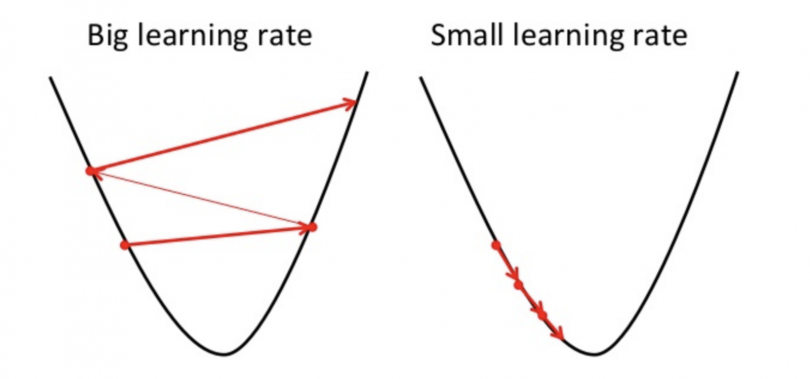
\includegraphics[width=.8\textwidth]{fig/L3/gradient-descent-learning-rate.png}
\end{figure}
 \end{frame}

\begin{frame}{Few comments}
\begin{itemize}[<+->]
\item The learning $\gamma$ is an important \alert{\bf hyperparameter} that needs to be tuned using, e.g random search
\item The key part of the formula is the computation of the gradient $\nabla L(\boldsymbol{\theta}_{k})$
\end{itemize}
\end{frame}


\section{Gradient backpropagation}
\begin{frame}{Training a neural-net: gradient backpropagation}

\begin{columns}

\column{.5\textwidth}
\begin{figure}
    \centering
 \begin{tikzpicture}[%
    node distance = 2.5em,
    basic/.style={draw,fill=blue!20,text width=1em,text badly centered},
    input/.style={basic,circle,fill=green!20},
    output/.style={basic,circle,fill=red!20},
    weights/.style={basic,rectangle},
functions/.style={basic,circle,fill=blue!10}
]
        \node[] (center) {};
        \node[right = of center, anchor = west,output] (right) {$\hat{y}$};
        \node[above of=center,functions] (h1) {$h_1$};
        \node[below of=center,functions] (h2) {$h_2$};
        \path[draw,->] (h1) -- node[above,midway]{$w^{1}_1$}(right);
        
        \path[draw,->] (h2) --  node[below,midway]{$w^{1}_2$}(right);
        
        \node[left = of h1, input] (x1) {$x_1$};
        \node[left = of h2, input] (x2) {$x_2$};
        
        \path [draw,->] (x1) -- node[above,midway]{$w^0_{11}$} (h1);
        \path [draw,->] (x1) -- node[pos=0.25,above]{$w^0_{12}$} (h2);
        \path [draw,->] (x2) -- node[pos=0.05,above]{$w^0_{21}$} (h1);
        \path [draw,->] (x2) -- node[below,midway]{$w^0_{22}$} (h2);
\end{tikzpicture}
\end{figure}
\begin{block}{Objective}
Determination of the best set of weights $\mathbf{w}$ to minimize the Loss function $L(\mathbf{w}) = ||\hat{y}(\mathbf{w})-y||^2$.\
\alert{Calculation of $\partial L/\partial w$}
\end{block}
\column{.6\textwidth}
\begin{enumerate}[<+->]
    \item Given a couple $(x,y)$
    \item \alert{Forward computation:}\\
    $h_j  =  f_0(\sum_{i=1}^2 w^0_{ij}.x_i)$\\
$\hat{y}  =  f_1(\sum_{j=1}^2 w^1_j. h_j)$
\item \alert{Compute the gradient of the loss:~}
$\boxed{\color{red}\partial L/\partial \hat{y}}$

    \item \alert{Gradient Backpropagation:}
    \begin{itemize}
   \item Layer 1\\
   $\alert{\partial L/\partial w_j^1} = 
   \boxed{\color{red}\partial L/\partial \hat{y}}.
   \partial f_1 / \partial w^1_j$\\
   
   $ \boxed{\color{blue}\partial L/\partial h_j} = 
    \boxed{\color{red}\partial L/\partial \hat{y}}. 
   \partial f_1 / \partial h_j$
   
   \item Layer 0\\
   $\alert{\partial L/\partial w^0_{ij}}=
  \boxed{\color{blue}\partial L/\partial h_j}
   .\partial f_1 / \partial w^0_{ij}  $
    
    \end{itemize}
\end{enumerate}

\end{columns}

\end{frame}


\section{Optimizing a machine learning (gradient method)}

\begin{frame}{Optimizing the loss}
    Several loss function (depending on the problem) can be defined.
    
    For example, Mean Square Error:
    
    \begin{alertblock}{Method}
    Find a minimum of L by adjusting the parameters (weights) $\mathbf{w}$ given the gradient of the loss with respect to the weights $\nabla_\mathbf{w}L$.
    \end{alertblock}
\end{frame}



\begin{frame}{Batch Vs Stochastic training}
Dataset: $(X,Y)$ with N samples denoted $(\mathbf{x_i},y_i)$

\begin{columns}[t]
\column{.56\textwidth}
\begin{footnotesize}
\begin{block}{Batch gradient:}\end{block}
    \begin{algorithmic}
    \Require{Learning rate(s): $\nu_k$}
    \Require{Initial weights: $\mathbf{w}$}
    \State $k \leftarrow 1$
    \While {stopping criterion not met}
   % \Require{NNNN}
    %\State Sample $m$ examples ($\mathbf{x}_i,y_i)$ from ($X,y$)
    \State Compute gradient: $\mathbf{g} \leftarrow \frac{1}{N}\sum_i^N\nabla_\mathbf{w}L(f(\mathbf{x}_i,y_i))$
    \State Update weights: $\mathbf{w} \leftarrow \mathbf{w} - \nu_k\mathbf{g}$
    \State $k \leftarrow k + 1$
    \EndWhile 
    \end{algorithmic}
    \end{footnotesize}
    \alert{1 Update / N forwards}
    \pause
    \column{.56\textwidth}
\begin{footnotesize}
\begin{block}{Stochastic gradient:}\end{block}
    \begin{algorithmic}
    \Require{Learning rate(s): $\nu_k$}
    \Require{Initial weights: $\mathbf{w}$}
    \State $k \leftarrow 1$
    \While {stopping criterion not met}
   % \Require{NNNN}
    %\State Sample $m$ examples ($\mathbf{x}_i,y_i)$ from ($X,y$)
    \State Sample an example ($\mathbf{x},y)$ from ($X,Y$)
    \State Compute gradient: $\mathbf{g} \leftarrow \nabla_\mathbf{w}L(f(\mathbf{x},y))$
    \State Update weights: $\mathbf{w} \leftarrow \mathbf{w} - \nu_k\mathbf{g}$
    \State $k \leftarrow k + 1$
    \EndWhile 
    \end{algorithmic}
    \end{footnotesize}
    \alert{1 Update / 1 forward}
    
    
    \end{columns}
\end{frame}

\begin{frame}{Mini-Batch training}
Dataset: $(X,y)$ with N samples
\begin{footnotesize}
\begin{block}{Mini-Batch gradient:}\end{block}

    \begin{algorithmic}
    \Require{Learning rate(s): $\nu_k$}
    \Require{Initial weights: $\mathbf{w}$}
    \State $k \leftarrow 1$
    \While {stopping criterion not met}
   % \Require{NNNN}
    \State Sample $m$ examples ($\mathbf{x}_i,y_i)$ from ($X,y$)
    \State Compute gradient: $\mathbf{g} \leftarrow \frac{1}{m}\sum_i^m\nabla_\mathbf{w}L(f(\mathbf{x}_i,y_i)$
    \State Update weights: $\mathbf{w} \leftarrow \mathbf{w} - \nu_k\mathbf{g}$
    \State $k \leftarrow k + 1$
    \EndWhile 
    
    \end{algorithmic}
    \end{footnotesize}
    \pause
        \alert{1 Update / $m$ forward}\\
        $m=1$: Pure stochastic gradient.\\
        $m=N$: Batch gradient

\end{frame}


%%%%%%%%%%%%%%%%%%%%%%
\begin{frame}{Let's have a break}
\url{https://playground.tensorflow.org}
\end{frame}



\section{Other regularization techniques}
%%%%%%%%%%%%%%%%%%%%%
\begin{frame}{Regularization}
\begin{block}{Definition:}
\alert{Regularization} refers to the \alert{set of techniques} that \alert{constraints} the optimization. It is generally used to \alert{avoid overfitting}, but can also be used to inject prior knowledge during the training phase (e.g. set known limits to parameters)
\end{block}
\pause
\begin{itemize}
    \item Stochastic mini-batch gradient is a regularization technique
\end{itemize}

\end{frame}

%%%%%%%%%%%%%%%%%%%%%
\begin{frame}{Early Stopping}
    \begin{figure}
        \centering
        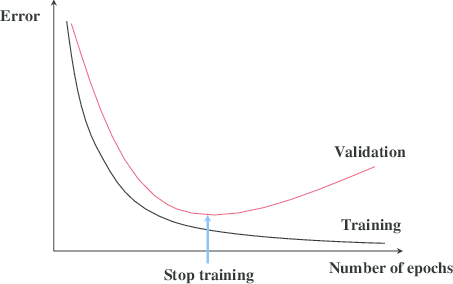
\includegraphics[width=\textwidth]{fig/L3/early_stopping.png}
    \end{figure}
\end{frame}
%%%%%%%%%%%%%%%%%%%%%
\begin{frame}{Dropout}
During training, randomly remove neurons on a layer with probability $p$.
 \begin{figure}
        \centering
\multiinclude[<+->][format=png,graphics={width=.6\textwidth}]{fig/L3/dropout}       
    \end{figure}
    \pause
    \begin{alertblock}{Practical remarks:}
    \begin{itemize}
        \item Avoid Dropout on convolutive layer
        \item Avoid Dropout on the last layer.
    \end{itemize}
    \end{alertblock}
    
    \end{frame}
    
    
\begin{frame}{Batch normalization}
From \textit{Ioffe et al. 2015, Batch normalizaion...}\\

Batch Normalization is a new type of layer.

If we use mini-batch training with a minibatch of size $m$:
\begin{columns}
\column{.8\textwidth}
\begin{footnotesize}
\begin{block}{Mini Batch Layer:}\end{block}
\renewcommand{\algorithmicrequire}{\textbf{Input:}}
\renewcommand{\algorithmicensure}{\textbf{Output:}}
    \begin{algorithmic}
    \Require{Values of $\mathbf{x_{1\dots m}}$}
    \Require{Initial parameters to be optimized: $\gamma, \beta$}
    \Ensure {$\mathbf{z_i} = {\rm BN}_{\gamma, \beta}(\mathbf{x}_i)$}
    \State $\mu \leftarrow \frac{1}{m}\sum_{i=1}^m \mathbf{x}_i$ \Comment{mini-batch mean}
    \State $\sigma^2 \leftarrow \frac{1}{m}\sum_{i=1}^m \left( \mathbf{x}_i - \mu \right)^2$ \Comment (mini-batch variance)
    \State $\hat{\mathbf{x}}_i \leftarrow (\mathbf{x}_i - \mu) / \sqrt{\sigma^2 + \epsilon}$ \Comment {normalize}
    \State $\mathbf{z_i} = \gamma \hat{\mathbf{x}}_i + \beta $ \Comment {Scale and shift}
    \State \Return $\mathbf{z_i}$
    \end{algorithmic}
    \end{footnotesize}

\end{columns}

$\mu$ and $\sigma^2$ are \alert{non-trainable parameters}. They are fixed for inferring new result (in test/validation).
\end{frame}

\section{Link with data assimilation}
\begin{frame}{Data Assimilation}
   Example of \textcolor{blue}{BLUE}{: Best Linear Unbiased Estimator}
    
    Given a state vector $\mathbf{x}\in \mathbb{R}^n$ and a data vector  $\mathbf{d}\in \mathbb{R}^m$:
\begin{tabular}{p{.3\textwidth}p{.2\textwidth}p{.2\textwidth}}
    $\mathbf{x}^{\rm f} = \mathbf{x}^{\rm t} + \mathbf{p},$ & $\overline{\mathbf{p}}=0,$ &$ \overline{\mathbf{p}\mathbf{p}^T} = \mathbf{C}_{xx}.$\\
    $\mathbf{d} = \mathbf{H}\mathbf{x}^{\rm t} + \boldsymbol{\epsilon},$ & $\overline{\boldsymbol{\epsilon}}=0,$ & $ \overline{\boldsymbol{\epsilon}\boldsymbol{\epsilon}^T} = \mathbf{C}_{\epsilon \epsilon}.$
    
    \end{tabular}
    \pause
    Estimating $\mathbf{x}^{\rm t}$ by minimizing the estimation error leads to minizing the following function:
    \begin{equation*}
        \mathcal{J}(\mathbf{x}) = 
          (\mathbf{d} - \mathbf{H}\mathbf{x})^T  \mathbf{C}_{\epsilon \epsilon}^{-1}  (\mathbf{d} - \mathbf{H}\mathbf{x}) + (\mathbf{x} - \mathbf{x}^{\rm f})^T \mathbf{C}^{-1}_{xx}(\mathbf{x} - \mathbf{x}^{\rm f})
    \end{equation*}
    \pause
    \begin{alertblock}{This is data assimilation!}
    We correct a forecast $\mathbf{x}^{\rm f}$ given some observational data $\mathbf{d}$
    \end{alertblock}
\end{frame}

\begin{frame}{Is it machine learning?}
\begin{footnotesize}

    \begin{itemize}
        \item Ridge regression: $
J(\bm{\theta}) =(\mathbf{y} - h_{\bm{\theta}}(\mathbf{x}))^T (\mathbf{y} - h_{\bm{\theta}}(\mathbf{x})) + \alpha  \theta^T \theta
$
\item BLUE:  $\mathcal{J}(\mathbf{x}) = 
          (\mathbf{d} - \mathbf{H}\mathbf{x})^T  \mathbf{C}_{\epsilon \epsilon}^{-1}  (\mathbf{d} - \mathbf{H}\mathbf{x}) + (\mathbf{x} - \mathbf{x}^{\rm f})^T \mathbf{C}^{-1}_{xx}(\mathbf{x} - \mathbf{x}^{\rm f})$
    \end{itemize}
    \end{footnotesize}
    \pause
    \begin{table}[]
        \centering
        \begin{tabular}{c|c}
            BLUE & Ridge \\
            \hline
            data $\mathbf{d}$ & target $\mathbf{y}$  \\
            Observation operator $\mathbf{H}$ & feature $\mathbf{x}$ \\
            State $\mathbf{x}$ & parameters $\bm{\theta}$\\
            $\mathbf{C}_{\epsilon \epsilon} \mathbf{C}^{-1}_{xx}$ & $\alpha$
        \end{tabular}
    \end{table}
    \pause
    \begin{block}{Further links...}
    If a numerical model is integrated over several time steps, it can be related to successive layers of a Neural Network.
    \end{block}
\end{frame}


\section{Probabilistic interpretation}
\begin{frame}{Maximum likelihood estimator and loss}
    We can assume that the observation $y$ follows a Gaussian law:
    $$
p(y/x) = \frac{1}{\sqrt{2\pi\sigma^2}}\exp -\frac{(y - \mu(x))^2}{2\sigma^2},
    $$
    where $x$ is observed and $\mu(x)$ is a function of $x$.\\
    
    Given a set of samples $(x_k,y_k)_{1:K}$, the negative log-likelihood is defined by
    
    $$
L = \sum_{k=1}^{K} \left(\frac{\log 2\pi\sigma^2}{2} + \frac{(y_k - \mu(x_k))^2}{2\sigma^2}\right)
$$

\alert{\bf Minimizing $L$ is maximizing the probability of having the observations $y_k$ given $x_k$.}
\end{frame}

\begin{frame}{Loss function of a neural net}
   \begin{block}{First case: $\sigma$ is constant}
   $\mu(x)$ is parametrized by a neural net $ G_\mu(x,{\boldsymbol \theta}_\mu)$\\
   The Maximum likelihood estimator is found by minizming:
   $$
L({\boldsymbol \theta}_\mu) =  \sum_{k=1}^{K} (y_k - G_\mu(x,{\boldsymbol \theta}_\mu))^2
$$
which is exactly the regression loss already introduced.
   \end{block}
\pause
{\footnotesize
\begin{block}{Second case:  $\sigma(x)$ is a function of $x$.}
In addition to $ G_\mu(x,{\boldsymbol \theta}_\mu)$, $\sigma(x)$ is parametrized by $G_\sigma(x,{\boldsymbol \theta}_\sigma)$.
The loss to minimize is then:
$$
L({\boldsymbol \theta}_\mu, {\boldsymbol \theta}_\sigma) = \sum_{k=1}^{K} \left(\frac{\log 2\pi G_\sigma(x_k,{\boldsymbol \theta}_\sigma)^2}{2} + \frac{(y_k - G_\mu(x_k,{\boldsymbol \theta}_\mu))^2}{2 G_\sigma(x_k,{\boldsymbol \theta}_\sigma)^2}\right)
$$
The neural net $G=(G_\mu,  G_\sigma)$ gives  also the uncertainty of its estimation in the form of the standard deviation.
\end{block}}
\end{frame}
\begin{frame}{Illustration}
\begin{figure}
    \centering
    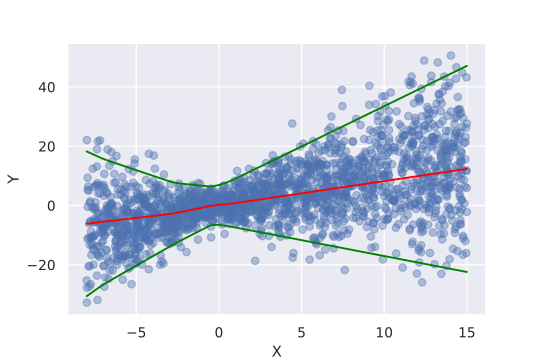
\includegraphics[width=.8\textwidth]{fig/L3/MLE.png}\\
    \textcolor{red}{In red the estimation of the mean $ G_\mu(x,{\boldsymbol \theta}_\mu)$}\\
    \textcolor{mygreen}{In green the confidence interval $ G_\mu(x,{\boldsymbol \theta}_\mu) \pm \sigma(x_k,{\boldsymbol \theta}_\sigma) $}
\end{figure}

\end{frame}


\section{A black box?}
%%%%%%%%%%%%%%%%%%%%
\begin{frame}{The black box paradigm}

The machine-learning based model is a \alert{black box}. It gives some results but we don't understand how.
\begin{figure}
    \centering
    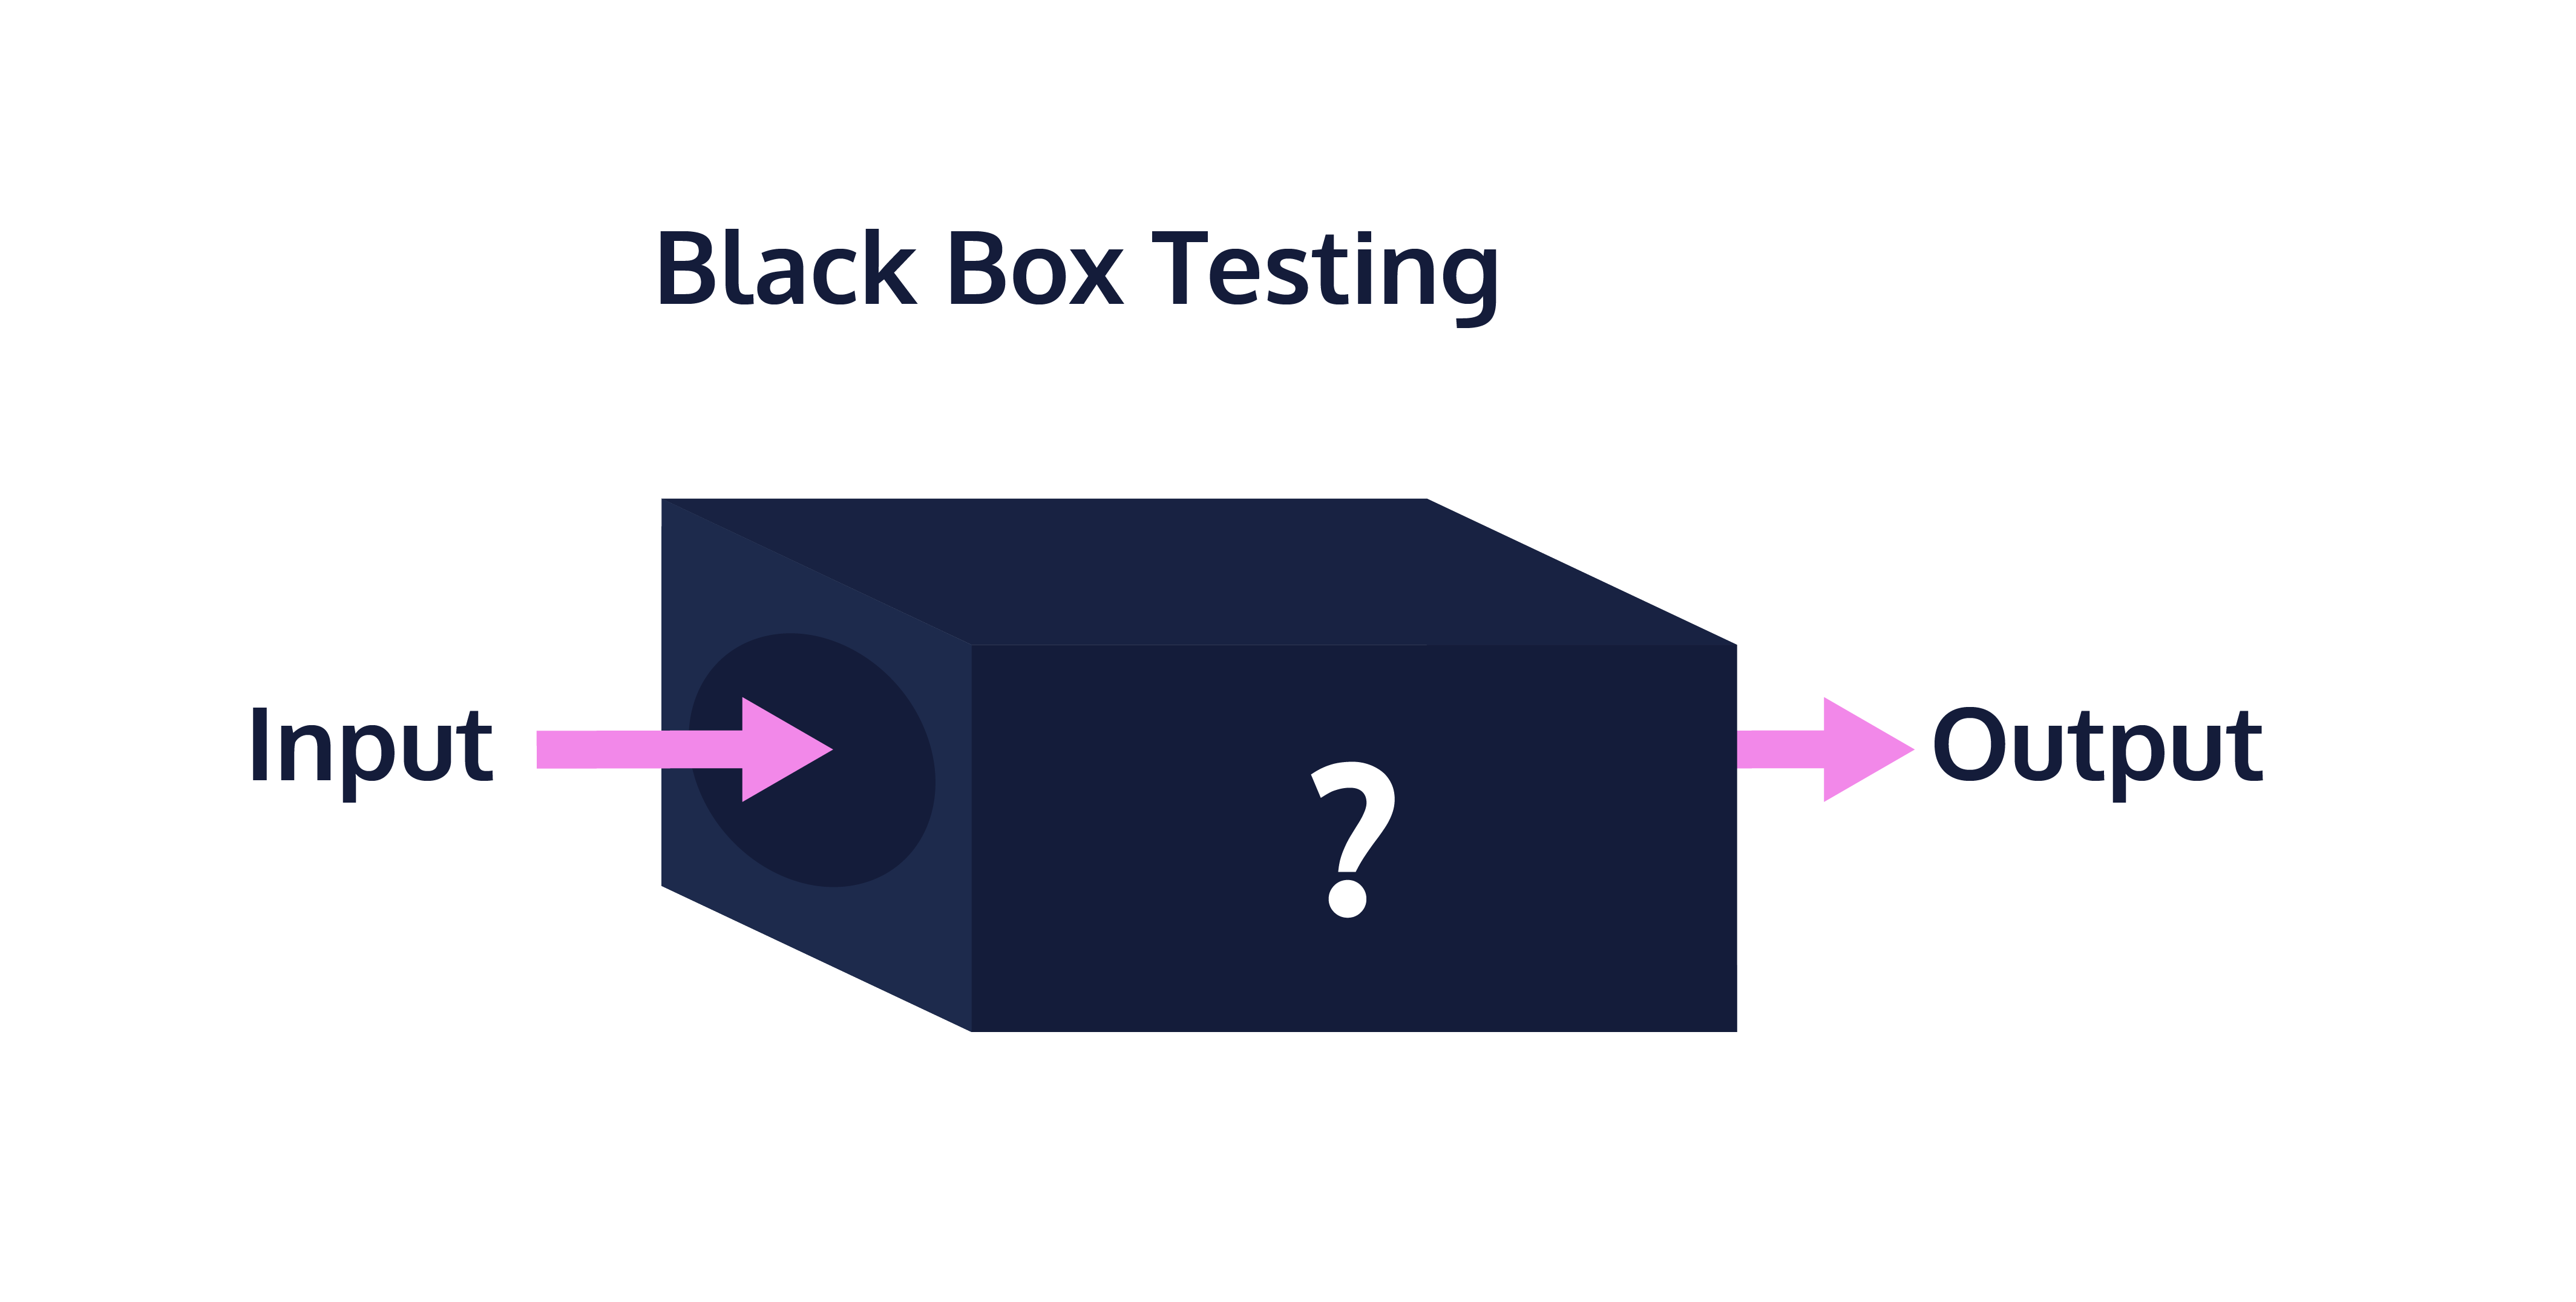
\includegraphics[width=.4\textwidth]{fig/L3/blackBox.png}

\end{figure}

\begin{columns}
\column{.5\textwidth}
{\bf Do we need to understand the model?}

\pause
{\it``Every time I fire a linguist, the performance of our speech recognition system goes up.''}

\rref[F. Jelinek, 1988]
\column{.5\textwidth}
\begin{figure}
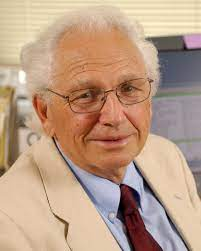
\includegraphics[width=.4\textwidth]{fig/L3/jelinek.jpeg}\\
  {\small {\it Frederick Jelinek 1932-2010}}
\end{figure}
\end{columns}

\end{frame}

%%%%%%%%%%%%%%%%%%%%
\begin{frame}{Beyond the black box}
\begin{block}{Motivation}
\begin{itemize}
    \item Build models that can be trusted
    \item Use other source of knowledge (e.g. physical properties) when data are not sufficient.
\end{itemize}
\end{block}

Two directions:
\begin{itemize}
    \item Add physical constraints to ML models
    \item Explainable/Transparent ML.
\end{itemize}


\end{frame}


%%%%%%%%%%%%%%%%%%%%
\begin{frame}{Add physical constraints to ML models}
\begin{itemize}
    \item \alert{Simple example}: enforce the positivity of some quantities (e.g. concentration)
    \item \alert{More complex}: enforce conservation laws\\
    {\small
Beucler, T., Pritchard, M., Rasp, S., Ott, J., Baldi, P. and Gentine, P., 2021. Enforcing analytic constraints in neural networks emulating physical systems. {\it Physical Review Letters}, 126(9), p.098302.}
\end{itemize}
\begin{columns}
\column{.6\textwidth}
\begin{figure}
    \centering
    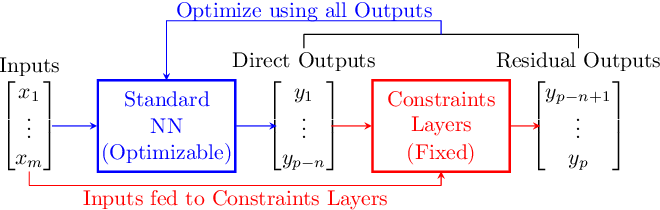
\includegraphics[width=\textwidth]{fig/L3/3-Figure2-1.png}\\
\rref[Beucler et al.]
\end{figure}
\end{columns}
\end{frame}

%%%%%%%%%%%%%%%%%%%%
\begin{frame}{Explainable/Transparent ML.}
The objective is to understand how the machine learning makes a prediction (e.g. which feature is important for the prediction).

\begin{columns}
\column{.4\textwidth}

{\footnotesize

    McGovern et al., 2019, Making the black box more transparent: Understanding the physical implications of machine learning. {\it Bulletin of the American Meteorological Society}\\
    \vspace{1em}

    Sonnewald  et al.,2021. Bridging observation, theory and numerical simulation of the ocean using Machine Learning. {\it Environ. Res. Lett.} 
    }
    

\column{.5\textwidth}
\begin{figure}
    \centering
    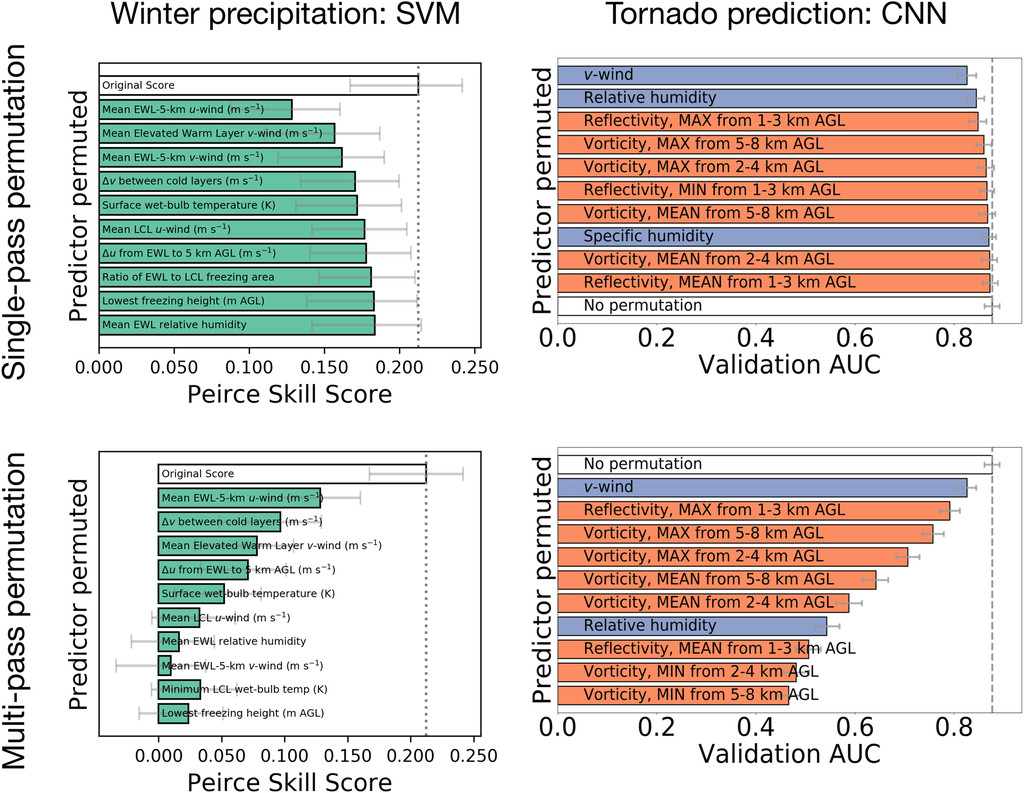
\includegraphics[width=.5\textwidth]{fig/L3/full-bams-d-18-0195.1-f3.jpg}\\
\rref[McGovern et al.]
\end{figure}
\end{columns}

\end{frame}



%%%%%%%%%%%%%%%%%%%%%
%%%%%%%%%%%%%%%%%%%%%
%%%%%%%%%%%%%%%%%%%%%
%%%%%%%%%%%%%%%%%%%%%
%%%%%%%%%%%%%%%%%%%%%%%%%%%%%%%%%%%%%%%%%%
%%%%%%%%%%%%%%%%%%%%%
%%%%%%%%%%%%%%%%%%%%%%%%%%%%%%%%%%%%%%%%%%

\end{document}

